% !Mode:: "TeX:UTF-8"
% 
% 编译说明
%		使用 XeLaTeX 编译引擎
%       TeX Live 的版本 2022 和 2021 目前都可以成功编译
%       如果使用 Overleaf 进行写作,请在左上角菜单中选择编译器为 XeLaTeX
%		在 MacBook 中推荐使用编译软件 Texpad


\documentclass[master]{bnuthesis}
	% bachelor/master/doctor: 学士/硕士/博士学位论文
	% twoside: 奇数页和偶数页页边距不一样,用于打印
	\usepackage{bnutils}
	% 调用宏包,使用 GB/T 7714-2015 参考文献著录格式
	\usepackage{gbt7714}
	
	\begin{document}
	\graphicspath{{figures/}}
	
	\frontmatter
	% !Mode:: "TeX:UTF-8"

\ctitle{越南高等教育外部质量保证体系研究}
\etitle{Research on External Quality Assurance System of Vietnamese Higher Education}


\makeatother

% 学士学位封面
% \cbuyuanxi{天文系} % 部院系
% \czhuanye{天文学} % 专业
% \cxuehao{201511160109} % 学号
% \cxueshengxingming{某某某} % 学生姓名
% \czhidaojiaoshi{某某} % 指导教师
% \czhidaojiaoshizhicheng{教授} % 指导教师职称
% \czhidaojiaoshidanwei{北京师范大学天文系} % 指导教师单位

% 博士(硕士)学位封面
\czuozhe{张氏越祯} % 作者
\cdaoshi{高益民\ 教授} % 导师
\cxibienianji{教育学部2019级} % 系别年级
\cxuehao{201939010022} % 学号
\cxuekezhuanye{比较教育学} % 学科专业
\cwanchengriqi{2025年7月} % 完成日期


% 中文摘要
\begin{cabstract}
本论文系统研究了越南高等教育外部质量保障体系在快速扩张、国际化和问责要求不断提高背景下的转型与挑战。研究背景源于越南高等教育在过去二十年间的迅猛发展:从2000年的约200所高校、100万学生,发展到2023年的近500所高校、超过250万学生。这种规模扩张在带来机遇的同时,也带来了质量保障的严峻挑战,特别是在确保教育质量与数量增长同步、满足劳动力市场需求、以及应对国际竞争压力等方面。

通过全面梳理全球与区域发展趋势,论文揭示了推动外部质量保障(EQA)机制发展的主要动力,特别是在东盟区域内。研究发现,全球高等教育质量保障呈现出从单一合规导向向多元化、适应性模式转变的趋势。传统的以政府主导、标准化评估为主的质量保障模式正在被更加灵活、注重持续改进和利益相关者参与的混合模式所替代。在东盟地区,这种趋势表现得尤为明显,各国在保持本土特色的同时,也在积极寻求区域合作与标准协调。

研究采用定性比较案例研究方法,深入分析了越南EQA体系的现状、成就与挑战。通过对越南教育部质量保障政策文件、评估报告和专家访谈的系统分析,研究识别出越南EQA体系在制度建设、评估机制、国际合作等方面的主要成就。同时,研究也揭示了体系存在的关键问题,包括评估标准不够细化、评估专家队伍能力不足、评估结果应用不充分、以及利益相关者参与度不高等。

为了提供更全面的分析视角,研究借鉴了中国国家主导模式和东盟大学联盟质量保障(AUN-QA)框架的经验。中国案例展示了国家强力主导的质量保障体系在实现大规模、快速变革方面的优势,但也凸显了如何在严格控制与学术创新自主权之间取得平衡的挑战。AUN-QA案例则体现了基于合作、共识和同行网络的区域质量保障模式的力量,证明了在多样化环境中无需单一权力机构集中控制也能建立共同标准。

论文运用现代管理与组织理论,包括新制度主义、利益相关者理论和委托代理理论,构建了适合越南国情的V-AQA混合与适应性模型。该模型基于五个核心要素构建:(1)领导与治理,强调战略导向和有效治理结构;(2)质量文化,注重建立持续改进的组织文化;(3)利益相关者参与,确保多方利益的有效整合;(4)内部流程,建立系统化的质量保障机制;(5)合作与协调,促进内部协作和外部合作。这五个要素相互关联、动态互动,形成了一个完整的质量保障生态系统。

研究结果指出,越南高等教育在规模扩张、资源分配和人才培养与劳动力市场需求之间仍面临诸多挑战。具体表现在:教育质量与数量增长不同步,优质教育资源分布不均,人才培养与就业市场需求脱节,以及国际竞争力有待提升等方面。这些挑战的根源在于质量保障体系的不完善,特别是在评估标准、专家队伍、结果应用和利益相关者参与等方面存在不足。

基于理论分析和国际比较,论文最终提出了以领导力、质量文化、利益相关方参与、内部流程和合作为核心的EQA体系综合改革模型。该模型强调:(1)建立多层次、协调统一的质量保障治理体系;(2)培育以质量为核心的组织文化;(3)构建多元利益相关者参与机制;(4)完善系统化的内部质量保障流程;(5)加强国内协作和国际合作。这一改革模型旨在提升体系效能,促进质量持续改进,助力越南高等教育更好地融入区域与全球教育体系。

研究的理论贡献在于构建了适合发展中国家高等教育质量保障的分析框架,丰富了质量保障理论在转型国家背景下的应用。实践意义在于为越南高等教育质量保障体系改革提供了系统性的政策建议,同时也为其他类似背景的国家提供了有价值的参考。研究结论强调,有效的质量保障体系不仅是一套流程的集合,而是一个复杂的生态系统,需要领导力、文化、利益相关者、流程和合作之间的动态平衡。
\end{cabstract}
\ckeywords{质量保障;高等教育;越南;外部质量保障;改革模型}

% English abstract
\begin{eabstract}
This dissertation investigates the transformation and challenges of Vietnam's higher education quality assurance system in the context of rapid expansion, international integration, and increasing demands for accountability. The research background stems from Vietnam's remarkable higher education development over the past two decades: from approximately 200 institutions and 1 million students in 2000 to nearly 500 institutions and over 2.5 million students in 2023. While this scale expansion has brought opportunities, it has also created serious quality assurance challenges, particularly in ensuring synchronized quality and quantity growth, meeting labor market demands, and responding to international competitive pressures.

Through a comprehensive review of global and regional trends, the study identifies the driving forces behind the development of external quality assurance (EQA) mechanisms, particularly in the ASEAN region. The research reveals that global higher education quality assurance is transitioning from single compliance-oriented approaches to diversified, adaptive models. Traditional government-led, standardized assessment quality assurance models are being replaced by more flexible approaches that emphasize continuous improvement and stakeholder engagement. This trend is particularly evident in the ASEAN region, where countries maintain their local characteristics while actively seeking regional cooperation and standard harmonization.

Using a qualitative comparative case study design, the research analyzes Vietnam's EQA system in depth, examining its current status, achievements, and challenges. Through systematic analysis of Vietnam's Ministry of Education quality assurance policy documents, evaluation reports, and expert interviews, the study identifies major achievements in Vietnam's EQA system regarding institutional development, evaluation mechanisms, and international cooperation. Simultaneously, the research reveals critical issues within the system, including insufficiently detailed evaluation standards, inadequate capacity of evaluation expert teams, insufficient application of evaluation results, and low stakeholder participation levels.

To provide a more comprehensive analytical perspective, the study draws lessons from China's state-driven model and the ASEAN University Network Quality Assurance (AUN-QA) framework. The China case demonstrates the advantages of a state-dominated quality assurance system in achieving large-scale, rapid transformation, but also highlights the challenge of balancing strict control with academic innovation autonomy. The AUN-QA case exemplifies the power of a regional quality assurance model based on cooperation, consensus, and peer networks, proving that common standards can be established in diverse environments without centralized control by a single authority.

The study applies modern management and organizational theories—including new institutionalism, stakeholder theory, and principal-agent theory—to construct the V-AQA hybrid and adaptive model, tailored to Vietnam's unique context. This model is built on five core elements: (1) Leadership and Governance, emphasizing strategic orientation and effective governance structures; (2) Quality Culture, focusing on establishing continuous improvement organizational culture; (3) Stakeholder Engagement, ensuring effective integration of multiple interests; (4) Internal Processes, establishing systematic quality assurance mechanisms; and (5) Cooperation and Coordination, promoting internal collaboration and external cooperation. These five elements are interconnected and dynamically interactive, forming a complete quality assurance ecosystem.

Findings highlight both achievements and persistent challenges, such as rapid scale growth, uneven resource distribution, and the gap between training outcomes and labor market needs. Specific manifestations include: asynchronous quality and quantity growth in education, uneven distribution of quality educational resources, disconnection between talent cultivation and employment market demands, and room for improvement in international competitiveness. The root causes of these challenges lie in the imperfection of the quality assurance system, particularly in areas such as evaluation standards, expert teams, result application, and stakeholder participation.

Based on theoretical analysis and international comparison, the dissertation concludes by proposing a comprehensive reform model for Vietnam's EQA system, emphasizing leadership, quality culture, stakeholder engagement, internal processes, and cooperation. This model emphasizes: (1) establishing a multi-level, coordinated quality assurance governance system; (2) cultivating quality-centered organizational culture; (3) constructing multi-stakeholder participation mechanisms; (4) perfecting systematic internal quality assurance processes; and (5) strengthening domestic collaboration and international cooperation. This reform model aims to enhance the system's effectiveness, support sustainable quality improvement, and facilitate Vietnam's integration into the regional and global higher education landscape.

The theoretical contribution of this research lies in constructing an analytical framework suitable for higher education quality assurance in developing countries, enriching the application of quality assurance theory in the context of transitional countries. The practical significance lies in providing systematic policy recommendations for Vietnam's higher education quality assurance system reform, while also offering valuable references for other countries with similar backgrounds. The research conclusion emphasizes that an effective quality assurance system is not merely a collection of processes, but a complex ecosystem requiring dynamic balance among leadership, culture, stakeholders, processes, and cooperation.
\end{eabstract}
\ekeywords{quality assurance; higher education; Vietnam; external quality assurance; reform model}



	\makecover
	
	\tableofcontents
	\listoffigures % 插图索引
	\listoftables % 表格索引
	
	\mainmatter
	\chapter{引言}
\label{chap:gioi_thieu}

\section{研究背景与选题理由}
\label{sec:boi_canh_ly_do}

\subsection{全球背景:质量保障成为必然趋势}

进入21世纪,高等教育(GDĐH)已超越其作为知识保存与传播场所的传统角色,成为决定各国竞争力和可持续发展的战略驱动力\footcite{Altbach2001}。在基于知识的全球化经济(knowledge-based economy)背景下,大学被视为"创新引擎",是培养高素质人力资源、产出科学技术发明以及为社会复杂挑战提供解决方案的场所\footcite{OECD_HE2008}。这一角色的转变对高等教育体系的质量提出了前所未有的紧迫要求。质量不再是学术象牙塔中的抽象概念,而已成为一个可衡量、可比较的因素,是国际舞台上激烈竞争的标准。

正是在这样的背景下,质量保障体系(ĐBCL - Quality Assurance),特别是外部质量保障(External Quality Assurance - EQA),已成为不可逆转的全球趋势。根据世界银行(World Bank)和联合国教科文组织(UNESCO)的报告,在过去几十年里,建立国家级质量保障机构的国家数量急剧增加,覆盖了全球几乎所有地区\footcite{WorldBank_QA_GlobalTrends}。这一强劲的扩散势头主要由三大动力推动:

\begin{enumerate}
    \item \textbf{高等教育的大众化 (Massification of Higher Education):} 学生规模和大学数量的爆炸性增长,包括私立院校的迅猛发展,使得高等教育体系变得前所未有的多样化和复杂化。这种多样性虽然带来了更多的教育机会,但同时也带来了质量下降和不均衡的风险。因此,政府和社会需要一个外部监督机制,以确保整个体系的最低质量门槛\footcite{Trow2007}。
    
    \item \textbf{问责制要求的提高 (Increased Demand for Accountability):} 随着公共财政和学习者对高等教育投入的日益增加,对大学问责制的要求也越来越高。包括政府、家长、学生和雇主在内的各利益相关方都想知道他们的投资是否带来了应有的效益。外部质量保障体系及其认证活动和结果公开,是履行这一问责制的最重要工具\footcite{Harvey2005}。
    
    \item \textbf{跨境教育的兴起 (Rise of Cross-border Education):} 全球化极大地促进了学生、教师和教育项目跨越国界的流动。这产生了对学位和学分互认的迫切需求。一个可靠的、其标准与国际惯例接轨的质量保障体系,是一个国家参与全球教育市场、吸引国际学生并确保本国学生文凭在国外获得承认的先决条件\footcite{Knight2006}。
\end{enumerate}

这些动力已将质量保障从一项纯粹的专业活动转变为一项重要的国家治理工具,是现代高等教育体系结构中不可或缺的要素。清晰理解这些全球趋势和动力,是准确分析像越南这样的特定国家质量保障体系所面临的背景与挑战的第一步。

\subsection{区域背景:东盟共同体内的质量协调化}
\label{subsec:boi_canh_khu_vuc}

如果说全球背景带来了竞争与融合的压力,那么区域背景则提出了合作与协调的要求。对越南而言,最重要的区域背景是东盟共同体。2015年东盟经济共同体(AEC)的成立设定了一个宏伟目标:建立一个统一的市场和生产基地,允许商品、服务、投资、资本以及特别是技术劳工(skilled labor)的自由流动\footcite{ASEAN_AEC_Blueprint}。

为实现这一目标,教育水平与质量的协调化及互认成为一项核心要求。在河内接受培训的工程师,需要具备与在曼谷或吉隆坡的雇主所承认的同等能力和文凭。深刻认识到这一要求,区域内的教育领导者们已率先努力建设一个共同的高等教育空间。实现这一努力最重要的工具是东盟大学网络(ASEAN University Network - AUN),特别是其下属的质量保障网络——AUN-QA(ASEAN University Network - Quality Assurance),该网络成立于1998年\footcite{AUNQA_History}。

AUN-QA并非一个具有强制权力的超国家认证机构,而是一个基于自愿、合作和同行学习(peer learning)原则运作的网络。其使命如官方文件所述,是"推动东盟高等教育机构的质量保障,提升高等教育质量,并为东盟共同体的共同利益与区域及国际机构合作"\footcite{AUN-QAGuide}。

AUN-QA的运作理念可概括为\textbf{"多元中的和谐"}原则。该网络不寻求消除各国教育体系之间的差异,而是建立一套共同的标准和评估流程,作为质量的"公分母"和通用语言。AUN-QA标准(目前是针对课程层级的4.0版)包含8项标准和明确的子标准,已成为该地区大学的重要参考框架。同行评审(peer review)流程,即由成员大学的专家相互评估,不仅有助于确保客观性,还创造了一个极其有效的经验和最佳实践分享机制\footcite{AUNQA_Report2023}。

对越南而言,积极参与AUN-QA网络具有战略意义。这不仅是提升国内大学质量和声誉的渠道,也是融入区域高等教育空间最快、最有效的途径。一个教育项目获得AUN-QA认证是其质量的重要保证,有助于该项目的毕业生在东盟劳动力市场上获得更多优势。因此,任何关于越南质量保障体系的分析都不能忽视AUN-QA框架作为区域背景重要因素的角色和影响。


\subsection{2015-2024年阶段越南高等教育发展背景:现状分析}

2015-2024年阶段标志着越南高等教育体系的一个重要转型时期。该体系已从注重扩大规模以满足社会学习需求,逐渐转向优先提升质量、调整结构和国际融合。分析此阶段的官方统计数据,将提供一幅全景图,突显越南高等教育所取得的成就、发展趋势以及面临的挑战,从而明确一个有效的外部质量保障体系产生的背景及其紧迫性。

\subsubsection{系统规模与结构的发展}

过去十年,越南高等教育最显著的特点之一是培养规模的急剧增长,而教育机构数量则在有控制地增长,体现了国家的战略导向。

\paragraph{关于教育机构数量:}
大学体系实现了稳定和可持续的发展。2015年,全国共有214所高等教育机构\footcite{stat_quy_mo_2015_2021},到2024年,这一数字增至\textbf{243所},其中包括176所公立大学和67所私立大学\footcite{stat_moet_2024}。近十年间仅净增约29所学校,表明政策不鼓励大规模新建学校,而是侧重于巩固和提升现有机构的质量。这为在整个体系内进行管理和质量保障工作创造了更有利的环境。

\paragraph{关于学生规模:}
与学校数量的稳定增长相反,学生规模实现了飞跃。大学生总规模从2015年的\textbf{175.3万}人猛增至2024年的\textbf{235.6万}人\footcite{stat_quy_mo_2015_2021}。这表明社会对大学学习的需求日益增长,高等教育体系已努力满足这一需求。

\begin{figure}
    \centering
    % Placeholder for the chart. Replace with your actual chart image.
    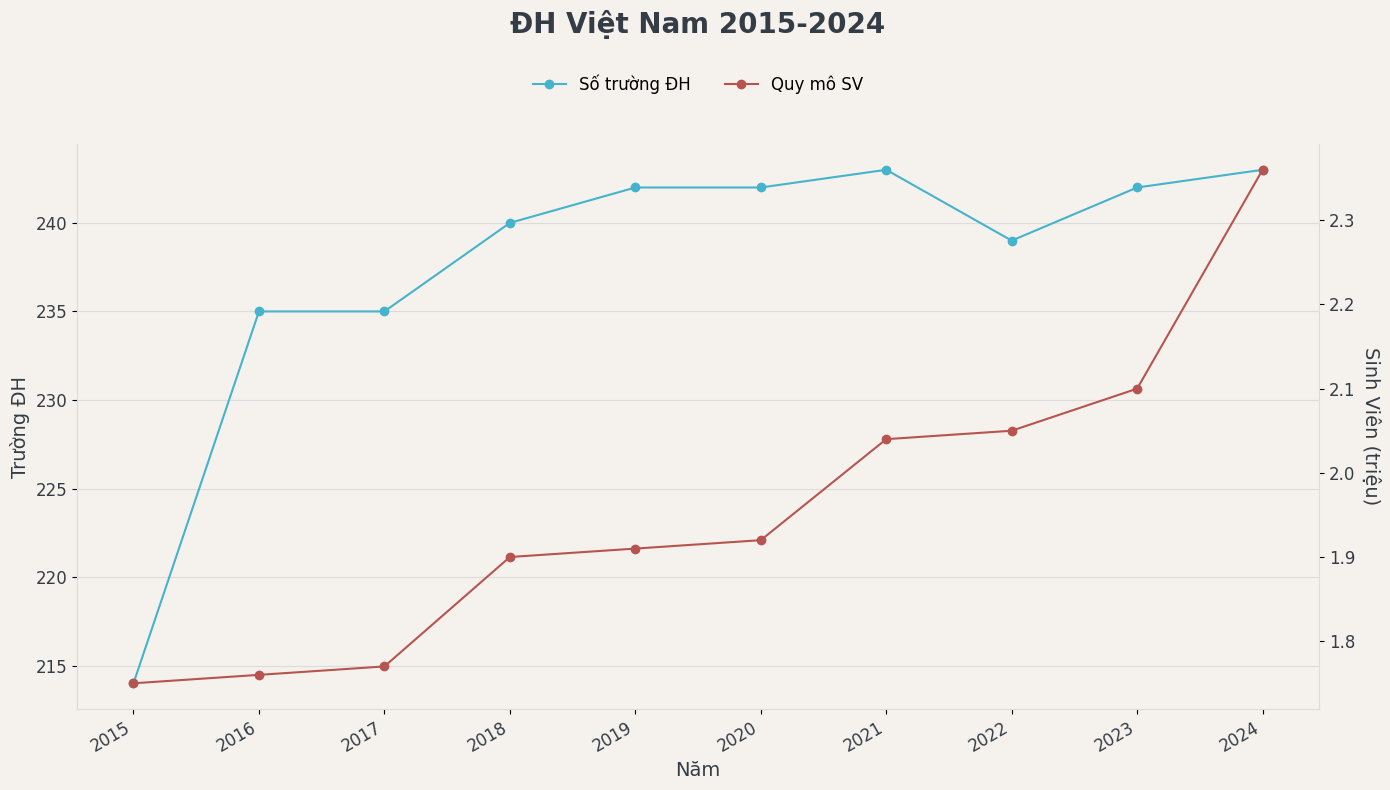
\includegraphics[width=0.9\textwidth]{image/bieu do 1 luan giao duc.png} 
    \caption{越南大学生规模与高校数量增长情况(2015-2024年)}
    \label{fig:quy_mo_phat_trien}
    \vspace{0.2cm}
    \footnotesize{\textit{来源:综合整理自越南教育培训部的数据\footcite{stat_moet_2024}及相关报告\footcite{stat_quy_mo_2015_2021}。}}
\end{figure}

特别是,2023-2024学年实现了突破性增长,比上一学年增加了\textbf{319,022}名学生\footcite{stat_moet_2024}。这并非寻常的线性增长,而是一次规模上的\textbf{飞跃(leap)},如图(图\ref{fig:quy_mo_phat_trien})所示。这种突增并非偶然现象,可以解释为多种政策和社会因素同时汇聚的结果,为整个体系带来了"推力"。

\paragraph{潜在原因分析:}
最直接和最重要的原因之一可能是各大学\textbf{招生政策的变化和招生指标的增加}。这一时期,除了传统的基于高中毕业考试成绩的录取方式外,多样化的录取方式也得到了大力发展。各大学加强使用学业成绩审查、自主能力评估考试等方式,为考生开辟了更多的"大门"。当大学,特别是民办大学和自主办学的公立大学,在确定招生指标和录取方式方面被赋予更多自主权时,它们倾向于扩大规模以满足社会需求和优化资源。整个体系招生指标的增加,结合灵活的录取方式,为前所未有的大量考生被录取和入学创造了条件。

第二个原因来自\textbf{经济社会因素和观念的转变}。COVID-19疫情后时期(2020-2022年)对劳动力市场和职业选择产生了一定影响。可能有一大部分学生和家庭意识到,对于没有高等专业水平的人来说,劳动力市场存在不确定性,从而坚定了大学文凭是未来稳定生活的必要"保险单"的信念。社会观念中"普及大学教育"的压力,推动了更大部分高中毕业生决定追求更高层次的学术道路,而不是进入劳动力市场或其他职业教育体系。

最后,这种突增是\textbf{共振效应}的结果。越南教育培训部扩大招生自主权的政策,如同一个"泄压阀",释放了社会长期以来积累的"需求压力"。当大学之门比以往任何时候都更加敞开时,大量的社会学习愿望在同一个学年得以实现,从而造成了规模上的飞跃。

然而,规模的快速增长也正是对质量保障工作的最大挑战。它提出了一个紧迫的问题:师资队伍、物质设施,特别是内部质量管理流程的发展,是否能跟上学生数量的增长速度?这正是现实背景,要求一个外部质量保障体系必须有效运作,既能监督,又能支持各大学克服这一挑战。

\paragraph{关于学生结构与民办院校的角色:}
民办大学的发展是教育社会化的一个亮点。就读于民办学校的学生比例已逐渐增加,从2015年的约20\%上升到2024年的\textbf{22.76\%},学生人数达到536,295人\footcite{stat_moet_2024}。这一数字不仅显示了私营部门日益重要的贡献,也表明越南已**提前实现了政府第35号决议中提出的到2025年民办学生比例达到22.5\%的目标**。民办院校的壮大创造了一个良性竞争的环境,推动公立学校不断创新和提高质量。

\subsubsection{招生工作现状与专业选择趋势分析}

分析招生数据不仅能展现体系的输入端情况,还能反映年轻一代的职业选择趋势,这是质量保障体系需要掌握并作出相应调整的重要因素。

\paragraph{参与比例与招生结果:}
近年来,参加高中毕业考试的考生数量一直稳定在100万以上\footcite{stat_thi_sinh_2024}。值得注意的是,申请大学录取的考生比例占了很大一部分,2024年约占参考考生总数的\textbf{68.5\%},显示进入大学仍然是大多数学生的首选。

被录取后确认入学的考生比例是反映培养项目吸引力和契合度的重要指标。在2022年短暂下降(80.34\%)后,该比例已恢复并于2024年达到\textbf{81.87\%},共有551,497名考生确认入学\footcite{stat_nhap_hoc_2024}。

% --- CHÈN BIỂU ĐỒ 2 ---
% --- CHÈN BIỂU ĐỒ (PHIÊN BẢN ĐÃ CẬP NHẬT) ---
\begin{figure}[h!]
    \centering
    % Thay thế bằng tên file ảnh mới bạn vừa tạo bằng Python
    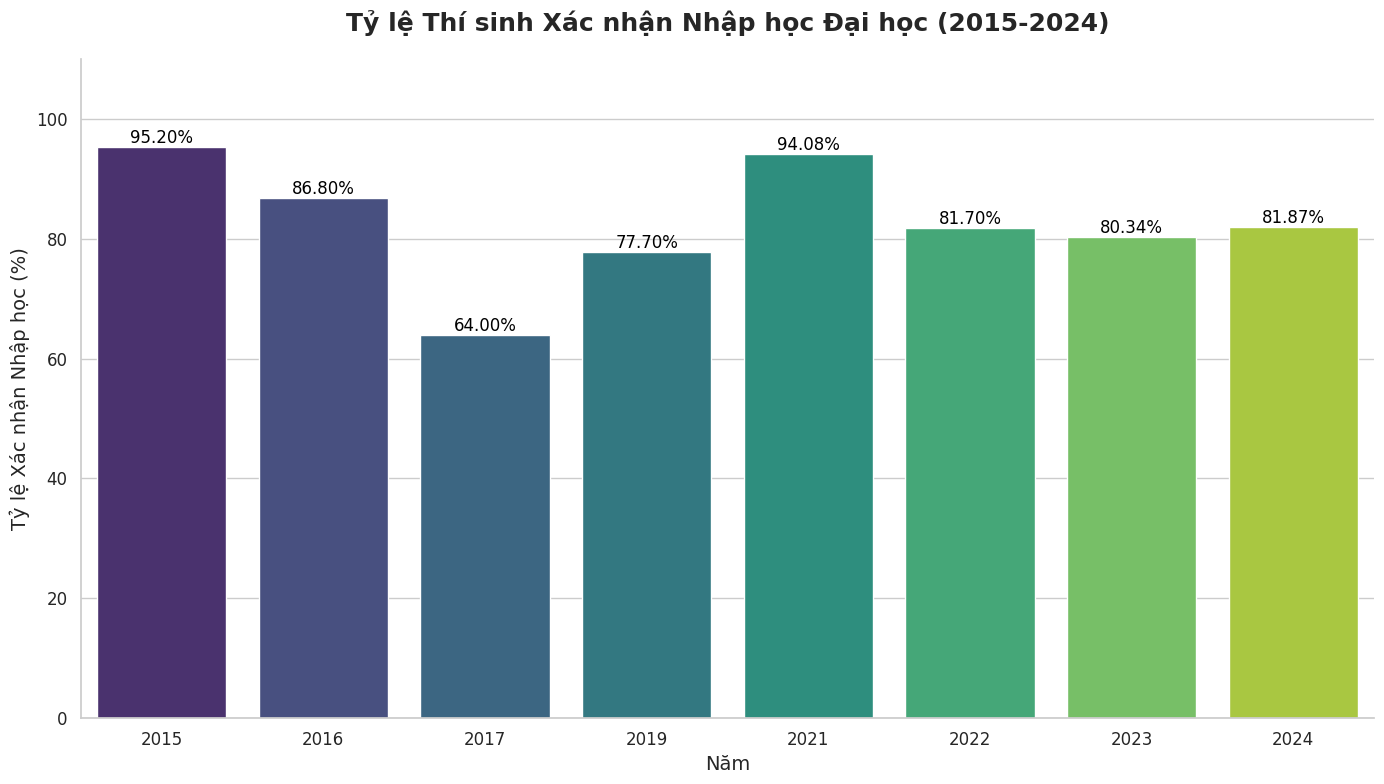
\includegraphics[width=0.8\textwidth]{image/ty_le_nhap_hoc_2015-2024.png}
    
    % Cập nhật caption cho đúng giai đoạn
    \caption{大学新生确认入学比例(2015-2024年)}
    \label{fig:ty_le_nhap_hoc_full}
    \vspace{0.2cm}
    
    % Cập nhật dòng nguồn với đầy đủ các trích dẫn
    \footnotesize{\textit{来源:综合整理自越南教育培训部及各新闻媒体历年数据 
    \footcite{ref1}\footcite{ref2}\footcite{ref3}\footcite{ref5}\footcite{ref7}\footcite{ref12}\footcite{ref19}\footcite{stat_nhap_hoc_2024}。}}
\end{figure}

这表明社会对高等教育体系的信心正在得到巩固。高入学率也意味着,平均每100名参加高中毕业考试的学生中,约有53人进入大学,这是过去9年来的最高比例,证实了越南已真正进入高等教育大众化阶段\footcite{stat_ty_le_vao_dh_2023}。

\paragraph{专业选择趋势:}
2024年的招生申请数据显示,专业选择趋势发生了显著变化。**教育科学与教师培养**类专业的志愿数量出人意料地大幅增长,比2023年增加了\textbf{85\%}。自然科学领域也吸引了大量关注,增幅达61\%\footcite{stat_tuyen_sinh_2024_so_lieu}。

相反,前些年的"热门"专业如**工商管理**(-3\%)和**计算机与信息技术**(-5\%)则出现了小幅下降趋势\footcite{stat_tuyen_sinh_2024_so_lieu}。这一转变可能反映了社会对长期人力资源需求的认知变化以及国家对教育行业的新政策。这是一个重要的信号,质量保障机构和各大学需要深入分析,以便及时调整培养结构。

\subsubsection{资源分析:师资队伍与物质设施}

一个教育体系的质量在很大程度上取决于其师资队伍的质量和保障条件。

\paragraph{关于师资队伍:}
2023-2024学年,全系统共有\textbf{88,031名全职教师}。在学历方面,有\textbf{28,862名教师拥有博士学位(占32.8\%)},49,229名教师拥有硕士学位(占55.9\%),其余为本科学历或其他学历\footcite{stat_moet_2024}。该学历结构如图\ref{fig:co_cau_giang_vien}所示。拥有博士学位的教师比例与前几年相比有了显著提高,这是提升培养和研究质量的重要前提。


% --- CHÈN BIỂU ĐỒ 3 ---
\begin{figure}[h!]
    \centering
    % Placeholder for the chart. Replace with your actual chart image.
    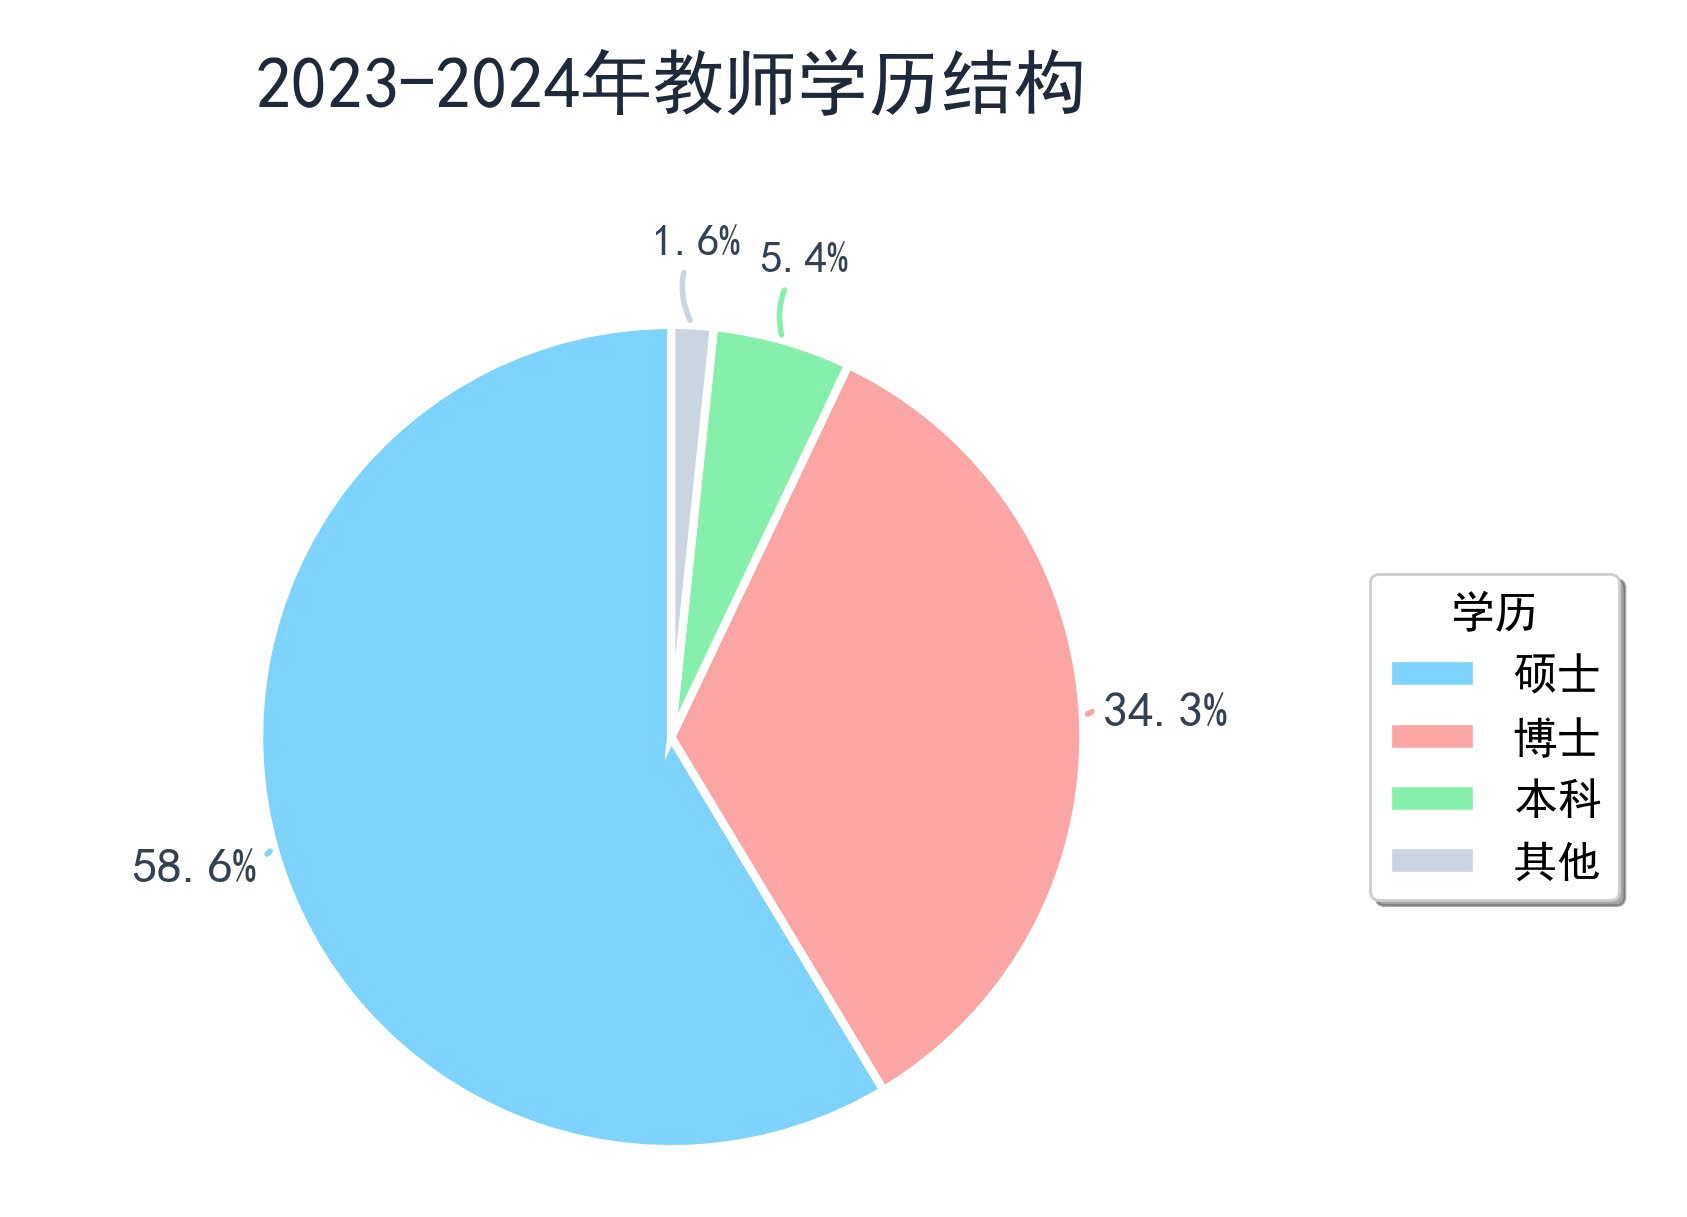
\includegraphics[width=0.6\textwidth]{image/co_cau_trinh_do_giang_vien_2023_2024.jpg}
    \caption{2023-2024学年全职教师学历结构}
    \label{fig:co_cau_giang_vien}
    \vspace{0.2cm}
    \footnotesize{\textit{来源:根据越南教育培训部数据计算\footcite{stat_moet_2024}。}}
\end{figure}

然而,生师比仍然偏高,尤其是在公立大学。全国平均生师比为公立大学30:1,民办大学22:1\footcite{stat_moet_2024}。公立大学的高生师比对确保师生之间有效互动(教育质量的核心要素)提出了巨大挑战。

\paragraph{关于资源分布:}
体系一个巨大且固有的挑战是地理分布上的严重不均衡。高质量的大学和师资队伍主要集中在红河三角洲(占学校总数的44.3\%)和东南部(18.4\%)两大重点经济区。而西原等贫困地区仅占学校总数的1.6\%\footcite{stat_quy_mo_2015_2021}。这种不平衡也明显体现在接受高等教育的机会上,红河三角洲的学生升入大学的比例(64.44\%)显著高于中北部山区(40.25\%)\footcite{stat_ty_le_vao_dh_2023}。这种差距要求质量保障政策必须考虑到地区因素,以确保公平和均衡发展。

\subsubsection{产出分析:毕业与就业}

产出质量是一个教育体系最终和最重要的衡量标准。
\begin{itemize}
    \item \textbf{毕业数量:} 2024年,高等教育体系为劳动力市场提供了\textbf{313,572名学士、工程师},与2023年的228,092人相比大幅增加\footcite{stat_moet_2024}。这表明高等教育在提供高水平人力资源方面扮演着越来越重要的角色。
    \item \textbf{就业情况:} 然而,这部分人力资源的质量仍然是一个问号。根据一份2018年的报告,毕业生毕业后就业率仅为\textbf{65.5\%}\footcite{stat_that_nghiep_2018}。更令人担忧的是,拥有大学、大专学历群体的失业率仍然高于中专学历群体。这表明所培养的技能与劳动力市场需求之间存在"不匹配"(mismatch),这是外部质量保障体系必须集中解决的核心问题。
\end{itemize}

\subsubsection{关于现状的初步结论}
对2015-2024年阶段统计数据的分析表明,越南高等教育正处于一个充满活力但又潜藏诸多挑战的发展阶段。
\begin{itemize}
    \item \textbf{成就:} 培养规模大幅扩展,满足了社会的学习需求;结构向民办领域积极转变;师资队伍的学历水平显著提高。
    \item \textbf{挑战:} 规模的急剧增长给质量带来了巨大压力;地区间资源分布不均的问题依然严峻;最重要的是,产出质量尚未能真正满足劳动力市场的要求。
\end{itemize}
这些挑战证实了建立一个强有力的外部质量保障体系的必要性,该体系不仅要监督合规性,还必须能够推动教育机构内部发生实质性变革,以解决质量和契合度的核心问题。


% done goi 2


\section{研究现状与研究问题综述}
\label{sec:tong_quan_nghien_cuu}

\subsection{研究背景与研究问题介绍}

如上文所分析,越南高等教育(GDĐH)的质量与质量保障问题及其挑战与机遇,近年来已引起众多学者、管理者和国际组织的关注。大量已发表的研究成果、政策报告和分析文章,为该领域构建了重要的知识基础。然而,一项新的研究要想做出真正的贡献,对现有成果进行系统化和批判性评估是不可或缺的一步。这一综述过程不仅旨在罗列已有的研究,更重要的是要识别那些"尚未探索的领域"、"悬而未决的问题"——换言之,即明确界定本论文旨在填补的\textbf{研究空白(research gap)}。

在此基础上,本论文确定其核心研究问题如下:

\begin{center}
\textit{一个在制度上不够强大、在适应变化背景方面不够灵活、在协调各相关方多样化要求方面不够全面的外部质量保障(ĐBCL)体系的缺失,正在对提升越南高等教育的实质性质量和国际竞争力的目标构成系统性障碍。}
\end{center}

为进一步阐明此问题,下文将从两大方面对相关研究进行综述:一是关于质量保障模型与理论的国际研究,二是以越南为具体背景的研究。

\subsection{关于质量保障模型与理论的国际研究综述}

世界范围内关于高等教育质量保障的研究经历了多个发展阶段,理论重心各不相同,为审视各国体系提供了丰富的视角。

在早期阶段,研究通常集中于描述认证机构的形成和结构,主要从公共管理和公共政策的角度出发。这些著作强调国家在制定规则和监督体系中的作用,这一方法接近于委托代理理论\footcite{Kivisto2008}。其重点在于阐明国家与大学之间的问责关系。

进入一个更发展的阶段,组织社会学家开始应用新制度主义理论来解释为何质量保障模式在全球范围内呈现出扩散和趋同的趋势。Meyer、Powell、DiMaggio的著作已成为经典,他们指出大学的行为不仅基于技术效率,还受到寻求在制度环境中获得合法性的强大压力\footcite{MeyerPowell2020}。后续如Kanwar等人(2019)的研究成功运用此理论框架,分析了在特定背景下推动应用质量保障的动力\footcite{Kanwar2019}。

近年来,随着质量保障体系变得日益复杂,研究者开始更多地关注不同主体之间的互动。利益相关者理论被越来越广泛地用于分析利益冲突以及将相关方(特别是学生和雇主)纳入质量保障流程的必要性。如Langrafe等人(2020)的研究提供了实证证据,表明利益相关者的参与与为学校和社会创造价值之间存在正相关关系\footcite{Langrafe2020}。

特别是,最新的研究已经认识到应用单一理论的局限性,并开始转向\textbf{综合与混合模型(hybrid models)}。欧洲大学协会(EUA)的报告经常强调从"控制"模式向"质量提升"模式的转变,其中外部评估流程旨在支持和促进内部的改进努力\footcite{EUA_Integration}。这种方法承认,一个有效的体系必须能够协调问责制和持续改进这两个目标。

\textit{从国际研究中得出的启示:}对国际文献的综述显示,关于质量保障的思维方式经历了明显的演变——从关注合规性控制,到解释制度压力,再到目前朝向综合、灵活和多方参与的模式发展。这表明,如果仅凭传统理论或仅描述政策规定来分析像越南这样的国家质量保障体系,将是不全面的。一个有深度的分析,需要将越南的体系置于这些理论和实践趋势的共同潮流中进行审视,同时识别其自身的独特性。



% done chuong 1 goi 3


\subsection{越南高等教育质量保障研究现状综述}
\label{subsec:tong_quan_vietnam}

在越南,高等教育质量与质量保障问题,已成为学术界和政策制定者高度关注的议题,尤其是在《高等教育法》颁布和修订之后。国内关于该领域的研究成果相当丰富,可分为三大类,每一类都有其独特的贡献与局限。

\paragraph{第一类:关于历史、政策与法律的研究。}
这是最普遍的研究类型,侧重于描述和系统化越南高等教育体系在各个时期的发展过程。黎文江(2003)等作者的著作,以及教育培训部各阶段的总结报告,为我们提供了从配给制时期到革新与融入时期的方针、政策变迁的全景视角\footcite{LeVanGiang2003}。这些研究在史料方面价值很高,有助于理解现行质量保障政策的出台背景。然而,这类研究的主要局限在于其方法主要是描述-统计性的。它们通常止步于"发生了什么",而未能从现代管理理论的视角深入探讨"为什么会这样发生"。因此,它们未能解释这些政策背后的制度动力、利益冲突或潜在的委托代理问题。

\paragraph{第二类:关于应用具体质量管理模型的研究。}
第二类研究包括关于在高等教育背景下应用具体质量管理模型的著作。陈庆德(2010)、阮德正(2002)等多位作者深入研究了全面质量管理(Total Quality Management - TQM)或ISO标准等模型\footcite{TranKhanhDuc2010}。这些研究具有很高的实践价值,为在教育机构内实施特定模型提供了详细的指导。然而,这些著作通常是"微观"或"技术性"的。它们通常孤立地审视某个管理模型,而未将其置于与整个外部质量保障体系(与认证中心、教育部的政策)的互动关系中。此外,它们更侧重于"如何应用",而非"为什么这个模型适合或不适合越南的组织文化和制度背景"。

\paragraph{第三类:关于教育机构认证现状的研究。}
第三类研究近年来发展迅速,侧重于分析具体大学或一组大学的质量认证工作现状。这些研究通常发表在国内专业期刊上,指出了各高校面临的许多实际困难和挑战,例如团队建设、证据收集或质量文化发展等问题\footcite{VJE_Challenges2023}。这些是极其宝贵的贡献,提供了生动的实证证据。然而,这些研究通常是"诊断性"的,并且是单一的案例分析。它们非常清楚地指出了问题的"症状",但通常未能深入分析导致这些症状的系统性"根源"。我们知道学校在数据方面遇到困难,但为什么这个问题具有普遍性和系统性?它是否源于治理结构、委托代理关系或制度压力?这些问题通常未被案例研究所透彻回答。

\subsection{研究空白的确定与本论文的研究方向}
\label{subsec:xac_dinh_khoang_trong}

通过对国内外研究流派的系统综述,一个重要的\textbf{研究空白(research gap)}被清晰地识别出来。具体而言,越南的研究虽然丰富,但仍存在三大主要局限:
\begin{enumerate}
    \item \textbf{缺乏一个综合的理论框架:} 现有的大多数研究要么是纯粹的政策描述,要么是应用单一的技术模型。极少有著作系统地运用现代管理与组织理论(如新制度主义、利益相关者理论、委托代理理论)来全面分析越南高等教育的质量保障体系。这导致分析往往停留在表面,未能触及塑造该体系的权力结构和潜在动力。
    
    \item \textbf{缺乏系统性的视角:} 研究通常聚焦于单个主体(国家、一所大学、一个管理模型),而缺乏一个整体的视角,未能将质量保障体系视为一个由众多主体和不同层次动态互动的复杂生态系统。这种系统性视角的缺失,使我们难以解释国际专家所指出的那些"恶性循环"(vicious cycles)和系统性问题。
    
    \item \textbf{侧重于"诊断"而非"模型构建":} 许多研究成功地指出了体系的"病症",但却未能提出一个基于坚实理论基础、具有整体性、可行性且论证严密的"治疗方案"。所提出的解决方案通常是零敲碎打的,解决的是个别症状,而非一个全面的改革模型。
\end{enumerate}

正是对这三个空白的清晰识别,确立了本论文的方向并彰显了其创新性。本论文的开展并非为了重复已有研究,而是要直接填补这些空白。本论文的目标不仅是描述现状,更是要通过一个综合的理论框架来\textbf{解释}这一现状,并在此基础上\textbf{提出}一个系统且可行的改革模型。通过构建和运用V-AQA模型,本论文将为越南高等教育在未来发展与融入阶段的外部质量保障体系改革问题,提供一个新视角、一个新分析工具和一个新方法。


% done goi 4

\section{研究目标、研究问题与研究意义}
\label{sec:muc_tieu_y_nghia}

在识别了越南高等教育(GDĐH)的"发展悖论"及既往研究中的空白后,本论文以明确的目标、具体化的尖锐研究问题展开,旨在为理论和实践两方面做出有意义的贡献。

\subsection{研究目标}
\label{subsec:muc_tieu_nghien_cuu}

本论文的研究目标是系统地建立理论与实证基础,以分析、评估并提出可行方案,旨在完善越南高等教育的外部质量保障(ĐBCL)体系,从而在国际一体化背景下,为解决规模增长与质量提升要求之间的矛盾做出贡献。

为实现上述总体目标,本论文将聚焦于以下四个具体目标:
\begin{enumerate}
    \item \textbf{系统化并构建理论框架:} 批判性地分析现代管理理论(新制度主义、利益相关者理论、委托代理理论)及世界先进的质量保障模型,从而构建一个适合越南特殊国情的综合分析框架——V-AQA模型。
    
    \item \textbf{分析与“诊断”现状:} 应用V-AQA理论框架,系统地分析越南外部质量保障体系的现状,识别其成就、核心挑战以及阻碍发展的系统性“瓶颈”。
    
    \item \textbf{借鉴国际经验教训:} 深入比较研究中国质量保障体系和AUN-QA框架这两个典型案例,从而在平衡控制与自主、区域标准与国家背景方面吸取宝贵的经验教训。
    
    \item \textbf{提出可行的模型与解决方案:} 基于理论基础和实证分析,详细提出混合与适应性质量保障模型(V-AQA)作为一个整体解决方案,并附上实施路线图及为越南管理者和政策制定者提供的具体政策建议。
\end{enumerate}

\subsection{研究问题}
\label{subsec:cau_hoi_nghien_cuu}

为引导研究过程并达成上述目标,本论文将集中回答以下三个主要研究问题:

\begin{enumerate}
    \item[\textbf{CQ1:}] \textbf{当前越南高等教育的外部质量保障体系在运行中呈现出哪些系统性的特点、成就与挑战?}
    \begin{itemize}
        \item \textit{子问题1a:} 主要参与方(教育培训部、认证中心、各大学)在体系中扮演何种角色,其互动关系如何?
        \item \textit{子问题1b:} 哪些核心“瓶颈”(在治理、文化、流程等方面)正在阻碍体系的有效性?
    \end{itemize}

    \item[\textbf{CQ2:}] \textbf{中国质量保障模型和AUN-QA框架的经验,为越南在平衡国家控制与大学自主、国际/区域标准与国情之间提供了哪些启示?}
    \begin{itemize}
        \item \textit{子问题2a:} 中国采取了哪些措施来既维持国家控制又促进国际竞争力,越南能从这种平衡中学到什么?
        \item \textit{子问题2b:} 在越南应用AUN-QA框架的过程中,将区域标准融入国家体系显示出哪些便利与挑战?
    \end{itemize}

    \item[\textbf{CQ3:}] \textbf{一个有效且适合越南国情的外部质量保障模型需要具备哪些核心组成部分和特性,其推行路线图应如何设计?}
    \begin{itemize}
        \item \textit{子问题3a:} 一个混合与适应性模型(V-AQA)的各组成部分应如何设计,以解决已识别的挑战?
        \item \textit{子问题3b:} 在实践中成功推行此模型需要哪些先决条件和政策解决方案?
    \end{itemize}
\end{enumerate}

\subsection{研究意义}
\label{subsec:y_nghia_nghien_cuu}

回答上述研究问题将在理论和实践两个层面带来重要的贡献。

\paragraph{理论意义 (Theoretical Significance):}
\begin{itemize}
    \item 本论文通过构建和验证一个\textbf{综合性理论分析框架(V-AQA模型)},为高等教育治理与质量保障的知识宝库做出贡献。该模型超越了单一理论的应用,提供了一个更全面的分析工具,尤其适用于研究发展中和转型期国家的高等教育体系。
    \item 本论文丰富了全球高等教育质量保障的案例研究。对越南体系与中国和AUN-QA进行深入分析和比较,将提供新的数据和视角,有助于国际学术界对质量保障模型的多样性和复杂性有更深入的理解。
\end{itemize}

\paragraph{实践意义 (Practical Significance):}
\begin{itemize}
    \item \textbf{对于政策制定者(教育培训部):} 本论文提供了对现行质量保障机制的优势、劣势及系统性问题的全面“诊断”。更重要的是,基于V-AQA模型的建议和方案,可以成为未来制定和完善与质量保障及大学自主相关的政策、通知、法令过程中的有益参考。
    \item \textbf{对于教育管理者(大学领导、认证中心):} 本论文提供了一套思维工具和一个行动框架,供各高校进行自我审视和评估其内部质量保障体系。关于质量文化、内部流程或利益相关者参与的分析,将有助于学校领导系统地识别需要优先改进的领域,而不是采取权宜之计。
    \item \textbf{对于学术界与社会:} 本论文有助于提高对越南高等教育质量问题的认识,并推动更深入的学术讨论,为政策对话提供科学论据,从而为建设一个高质量和可持续的越南高等教育体系的共同目标做出贡献。
\end{itemize}


% done chuong 1 goi 5


\section{研究对象、范围与论点}
\label{sec:doi_tuong_pham_vi_luandiem}

为确保研究的可行性、深度和焦点,明确界定研究对象、范围并提出核心论点是先决条件。这些要素将决定整个研究工作的界限和重点。

\subsection{研究对象与范围}
\label{subsec:doi_tuong_pham_vi}

\paragraph{研究对象:}
本论文的核心研究对象是\textbf{越南高等教育(GDĐH)的外部质量保障(External Quality Assurance - EQA)体系}。该对象被理解为一个复杂的生态系统,包括三大主要组成部分:
\begin{enumerate}
    \item \textbf{参与者 (Actors):} 包括政策制定机构(主要是教育培训部)、认证执行组织(国内各教育质量认证中心及获准的国际/区域组织)以及高等教育机构(作为体系影响的对象)。
    \item \textbf{结构与机制 (Structures and Mechanisms):} 包括法规文件、评估标准体系、认证流程以及相关的财政、政策机制。
    \item \textbf{互动关系 (Interactions):} 包括上述参与者之间的权力、问责和合作关系。
\end{enumerate}

\paragraph{研究范围:}
为确保可行性和深度,本论文的研究范围限定如下:
\begin{itemize}
    \item \textbf{内容方面:} 研究主要集中于\textit{外部质量保障(EQA)}。各大学的内部质量保障(Internal Quality Assurance - IQA)方面虽会提及,但主要是在其作为EQA总体体系中受影响的对象和组成部分的角度,而不会深入分析某一具体学校的IQA流程。
    
    \item \textbf{时间方面:} 尽管会回顾历史进程,但本论文将重点分析自\textbf{2012年至今}的政策与实践。选择2012年为起点,是因为该年《高等教育法》首次颁布,标志着越南质量保障体系制度化建设的一个重要转折点。这一时期有助于研究捕捉到体系最新的变化与挑战。
    
    \item \textbf{空间方面:} 研究以\textbf{越南}为中心分析案例(central case)。为获得比较视角并汲取经验,本论文将选用两个有选择性的比较案例:\textbf{中国的质量保障体系}(代表由国家强力主导的国家模式)和\textbf{AUN-QA框架}(代表对越南有直接影响的区域合作模式)。
\end{itemize}

\subsection{论文的核心论点}
\label{subsec:luan_diem_chinh}

基于全部背景、研究空白和已确定的目标,本论文将捍卫并证明以下核心论点:

\begin{quote}
\textit{\textbf{
本论文论证,越南高等教育外部质量保障体系所固有的、系统性的挑战——其体现为规模增长与质量停滞、自主诉求与严格管控之间的矛盾——无法通过零散的政策解决方案或机械地套用国际模式来解决。相反,它们需要一种全面、综合且对具体国情高度敏感的方法。
}}

\textit{\textbf{
因此,本论文提出并证明,混合与适应性质量保障模型(V-AQA),及其五个核心要素——(1)领导与治理、(2)质量文化、(3)利益相关者的参与、(4)内部流程以及(5)合作与协调,是重构该体系最合适的理论框架和实践方案。推行此模型有能力解决其内在矛盾,促进一种内生的质量文化,从而可持续地提升高等教育质量,并帮助越南有效融入区域及全球教育空间。
}}
\end{quote}

该论点是贯穿始终的主线,是整个研究工作的灵魂。本论文的后续章节,从现状分析、国际比较到方案建议,都将为捍卫这一核心论点提供理论和实证依据。

% done chuong 1 goi 6

\section{方法论与研究方法}
\label{sec:phuong_phap_luan}

为回答已提出的研究问题并验证核心论点,本论文采用了一套系统设计的科学方法论,并结合了多种具体的研究方法。本部分将详细阐述研究哲学、研究路径、总体研究设计,以及将要使用的数据收集与分析方法。

\subsection{研究哲学与研究路径}
\label{subsec:triet_ly_tiep_can}

每一项科学研究都由一套关于现实本质(本体论 - ontology)和知识本质(认识论 - epistemology)的基础性假设所引导。明确这些假设有助于确定合适的研究方法并确保整个研究的一致性\footcite{Creswell2018}。

本论文基于\textbf{建构主义(Constructivism)}的哲学基础。该哲学认为,社会现实并非独立于外部存在的客观事物,而是通过人们的互动、诠释及赋予其的意义而被“建构”(constructed)出来的\footcite{GubaLincoln1994}。应用于本课题,“教育质量”或“质量保障体系的有效性”并非单一、客观的真理,而是一个复杂的概念,由不同主体(国家、学校、学生、企业)的视角、利益和互动所塑造。因此,要理解质量保障体系,研究需要深入探究该体系中各主体的背景、流程和多样化的诠释。

基于此哲学基础,本论文主要采用\textbf{定性研究方法(qualitative approach)}。定性方法特别适用于本课题,原因如下:
\begin{itemize}
    \item \textbf{探索深度与复杂性:} 质量保障中的政策、治理和组织文化等问题是复杂、多维的,难以简单量化。定性方法允许研究者深入问题的本质,探索精细的因果关系和独特的背景因素\footcite{Yin2018}。
    \item \textbf{解释意义与诠释:} 定性研究不仅衡量“发生了什么”,更侧重于解释“为什么”和“如何”发生。它允许分析不同主体的诠释、观点和动机,而这正是理解一个社会系统运作的核心要素。
    \item \textbf{从实践中构建理论:} 这种方法非常适合本论文不仅要验证还要构建新理论模型(V-AQA)的目标。通过深入分析实践数据,研究可以提炼出概念、关系,并构建一个有坚实实践基础的理论框架(扎根理论方法)\footcite{Charmaz2006}。
\end{itemize}

\subsection{研究设计}
\label{subsec:thiet_ke_nghien_cuu}

为实现定性研究路径,本论文采用\textbf{比较案例研究设计(comparative case study design)}。选择此设计是因为它允许研究者在真实情境中对一个当代现象进行深入的、实证性的调查,特别是当现象与情境之间的界限不明确时\footcite{Yin2018}。

在此设计中,各个“案例”(cases)是有目的地选择的,以服务于研究目标,具体如下:
\begin{itemize}
    \item \textbf{主要案例,深度研究(In-depth, Primary Case):越南的外部质量保障体系。} 这是整个论文的核心。深入研究此案例旨在全面“诊断”其现状、动因、挑战以及各主体之间复杂的互动关系。
    
    \item \textbf{比较案例(Comparative Cases):}
    \begin{enumerate}
        \item \textbf{中国的质量保障体系:} 被选为比较案例,因为它代表了一种“强国家”模式,集中化,在政治社会结构上与越南有许多相似之处,但规模和发展水平不同。与中国的比较有助于吸取在平衡控制与竞争方面的经验。
        \item \textbf{AUN-QA的质量保障框架:} 被选中是因为它是对越南影响最直接、最强烈的区域模式。它代表了一种基于网络、同行合作的方法,与国家的集中模式形成对比。分析AUN-QA有助于吸取在协调标准和区域一体化方面的经验。
    \end{enumerate}
\end{itemize}

使用多案例比较设计(multiple-case study)带来了许多优势。它不仅有助于阐明主要案例(越南)的独特性,还使研究者能够得出具有更高分析性概括(analytic generalization)能力的结论,而不是仅仅局限于单一情境的结论\footcite{Yin2018}。

研究过程将按以下逻辑阶段展开:
\begin{enumerate}
    \item \textbf{第一阶段:构建理论框架。} 这正是第二章的内容,在此阶段建立V-AQA分析模型。
    \item \textbf{第二阶段:为每个案例收集和分析数据。} 使用具体方法(将在下文介绍)为每个案例(越南、中国、AUN-QA)收集和分析数据。
    \item \textbf{第三阶段:跨案例分析(Cross-case Analysis)。} 基于V-AQA分析框架,对比和比较三个案例的发现,从而确定异同点并总结经验教训。
    \item \textbf{第四阶段:综合与模型构建。} 基于全部分析结果,完善并详细提出V-AQA模型,作为对越南可行的解决方案。
\end{enumerate}

此研究设计确保了严谨性和逻辑性,使本论文能够系统且有说服力地从理论走向实践,从分析走向建议。


% done chuong 1 goi 7


\subsection{数据收集与分析方法}
\label{subsec:phuong_phap_cu_the}

为执行已提出的比较案例研究设计,本论文将主要依赖通过定性研究方法对二手数据(secondary data)的收集与分析。多种方法的结合将有助于增强研究结果的有效性和可靠性(三角互证法)\footcite{DenzinLincoln2011}。

\subsubsection{文献分析法}
\label{subsubsec:phan_tich_tai_lieu}

这是本论文\textbf{最主要、最重要的}数据收集与分析方法。文献分析是一个系统性的过程,用以审阅和评估印刷版及电子版的文献,旨在提炼意义、收集信息并形成实证证据\footcite{Bowen2009}。此方法特别适用,因为它允许接触丰富、稳定且无反应性(non-reactive)的数据源,帮助研究者在不影响被研究对象的情况下分析政策和实践。

将收集和分析的主要文献来源包括三类:
\begin{enumerate}
    \item \textbf{法规与政策文件类:} 这些是官方文件,为质量保障体系提供了法律框架。
    \begin{itemize}
        \item \textit{越南案例:} 《教育法》(2019年)、《高等教育法》(2012年)及其补充修订法案(2018年);政府的相关法令;教育培训部关于颁布课程标准、质量评估标准以及规定认证中心组织与活动的通知和决定。
        \item \textit{中国与AUN-QA案例:} 中国教育部的相应文件,AUN-QA的官方指导文件(《AUN-QA评估指南》)。
    \end{itemize}
    
    \item \textbf{报告与评估文件类:} 这些是“鲜活的”文件,反映了体系的实际运作情况。
    \begin{itemize}
        \item 越南部分代表性大学在参与认证时提交的自评报告(Self-Assessment Reports - SAR)。
        \item 认证中心对各大学的外部评估报告(External Assessment Reports)。
        \item 世界银行(World Bank)、亚洲开发银行(ADB)等国际组织及其他发展合作伙伴(如英国文化协会)的分析、评估报告。
        \item 教育培训部及各大学的学年总结报告、项目方案、发展战略。
    \end{itemize}
    
    \item \textbf{学术与档案文件类:} 包括已发表的研究成果。
    \begin{itemize}
        \item 国内外专业期刊上的科学论文。
        \item 关于高等教育质量保障的国内及国际研讨会论文集。
        \item 已通过答辩的相关博士、硕士论文。
        \item 权威媒体上的政策分析与评论文章。
    \end{itemize}
\end{enumerate}

分析过程将采用\textbf{主题内容分析法(thematic content analysis)}。来自文献的数据将被编码、分类,并按照V-AQA理论框架的五个要素(领导与治理、质量文化等)预设的主题进行整理。这种方法有助于确保数据分析的系统性,并直接服务于回答研究问题\footcite{BraunClarke2006}。

\subsubsection{历史分析法}
\label{subsubsec:phan_tich_lich_su}
历史分析法将被用于重构越南外部质量保障体系的演进过程。这不仅是按时间顺序叙述事件,更是旨在解释特定历史社会背景下政策的变迁与延续性\footcite{Tosh2015}。通过分析从“革新”时期至今的质量保障政策,此方法将有助于回答以下问题:
\begin{itemize}
    \item 某一特定政策为何在那个时间点出台?
    \item 哪些经济、政治、社会因素影响了质量保障体系的变革?
    \item 旧政策留下了哪些影响至今体系的“遗产”(legacies)?
\end{itemize}
采用此方法有助于研究获得历史深度,避免对质量保障体系采取静态和脱离背景的视角。

\subsubsection{比较分析法}
\label{subsubsec:phan_tich_so_sanh}
如研究设计中所述,比较分析法扮演着核心角色。这并非随意的比较,而是基于明确分析框架的有目的、系统性的对比\footcite{Sartori1991}。
\begin{itemize}
    \item \textbf{比较目的:} 并非为了给体系排名“优劣”,而是为了:(1)通过与其他体系的对比,突显越南体系的独特性和特殊性;(2)为越南国情吸取可行的经验教训和可应用的普适原则。
    \item \textbf{比较框架:} 为避免肤浅的比较,本论文将直接使用包含五个要素的\textbf{V-AQA模型}作为对比框架。例如,比较章节将分析:越南的\textit{领导与治理}要素与中国有何不同?越南的\textit{内部流程}要素可以从AUN-QA框架中学到什么?
    \item \textbf{比较逻辑:} 本论文将应用“最相似系统,不同结果”(most similar systems, different outcomes)和“最相异系统,相似结果”(most different systems, similar outcomes)的逻辑,以找出关键的解释性因素\footcite{PrzeworskiTeune1970}。
\end{itemize}

\subsubsection{理论综合与模型构建法}
\label{subsubsec:xay_dung_mo_hinh}
这是一种创造性的方法,体现了本论文的核心贡献。它包括以下步骤:
\begin{enumerate}
    \item 批判并指出既有理论的局限性。
    \item 从不同理论中综合关键概念和关系。
    \item 构建一个具有明确定义组成部分和关联的新模型(V-AQA)。
    \item 运用该模型分析实践数据并验证其有效性。
\end{enumerate}
此方法使本论文不仅是理论的“消费者”,更是在小范围内成为新理论工具的“创造者”,为该研究领域的发展做出贡献。

这四种方法的娴熟结合,将确保本论文能够全面地回答研究问题,其论点既有理论深度,又有丰富的实证证据支持。

% done chuong 1 goi 8


\section{核心概念}
\label{sec:khai_niem_cot_loi}

为确保整篇论文的清晰、一致和准确,明确定义核心概念是一项强制性要求。本部分将重点阐明贯穿全文使用的中心术语,包括:“高等教育质量”、“质量保障”,以及“外部质量保障”与“认证”之间的关系。

\subsection{高等教育中的质量:一个多维度的概念}
\label{subsec:khai_niem_chat_luong}

“质量”是高等教育研究中争议最多、也最难把握的概念之一。它并非一个单一、静止的概念,而是具有多维度、依情境和不同利益相关者视角而变化的特性。Harvey和Green(1993)在一篇经典著作中确定了五种不同的定义质量的方法,有助于阐明这一概念的复杂性\footcite{HarveyGreen1993}:

\begin{enumerate}
    \item \textbf{作为卓越的质量 (Quality as Exceptional):} 这是传统观点,认为质量是某种特殊的、高级的东西,仅存于少数精英教育机构中。在此视角下,质量等同于超越最高标准,难以广泛实现。
    
    \item \textbf{作为完美的质量 (Quality as Perfection or Consistency):} 此观点受工业生产领域影响,将质量定义为“零缺陷”(zero defects)并始终如一地满足既定技术参数。它强调流程和合规性。
    
    \item \textbf{作为合目的性的质量 (Quality as Fitness for Purpose):} 这是最具影响力的定义之一。质量的评估基于一个教育机构或一个培养项目在多大程度上实现了其自行宣布的目标和使命。一所职业学校如果出色地完成了培养熟练技工的目标,即便它不是顶尖研究机构,也可以被认为是高质量的。
    
    \item \textbf{作为物有所值的质量 (Quality as Value for Money):} 从支付方(政府、家长、学生)的角度来看,质量通过投资效益的视角来审视。一个高质量的项目是其带来的收益(例如:就业机会、高收入)与其投入成本相称或更大的项目。这种方法强调财务问责。
    
    \item \textbf{作为转化的质量 (Quality as Transformation):} 这是一个具有深刻教育意义的观点,聚焦于学习者。质量被定义为教育过程为学习者创造积极变化、转化的能力——不仅在知识、技能方面,还在思维、认知和价值观方面。这是为学生“创造附加值”(value-added)的过程。
\end{enumerate}

认识到这种多维度性,本论文将不选择单一的定义,而是采用一种\textbf{综合性观点}。据此,\textbf{高等教育中的质量}被理解为教育机构在以下方面的能力:\textit{(1)实现其已公布的目标和已承诺的最低标准(合目的性);(2)满足并为主要利益相关者,特别是学习者和社会创造价值(转化与物有所值);以及(3)持续改进流程以可持续地维持和提升这些价值。}

\subsection{质量保障与认证:区别与关系}
\label{subsec:khai_niem_dbcl_kd}

在关于质量的讨论中,“质量保障”(Quality Assurance - QA)和“认证”(Accreditation)这两个术语常被交替使用,但实际上它们的含义不同,并存在包含关系。

\paragraph{质量保障 (Quality Assurance - QA):}
质量保障是一个更宽泛的概念,具有流程性和系统性。根据国际高等教育质量保障机构网络(INQAAHE)的定义,质量保障是“为建立对质量得到维持和提升的信心所必需的所有政策、流程、计划性行动和系统”\footcite{INQAAHE_Glossary}。
因此,质量保障包括一所大学为管理其质量而进行的所有活动,从课程设计、招生、教学、学生评估,到收集反馈和实施改进。它包含两个方面:
\begin{itemize}
    \item \textbf{内部质量保障 (Internal Quality Assurance - IQA):} 是指由教育机构自身建立和运行的、用以自我监控和改进其质量的全部机制和流程。
    \item \textbf{外部质量保障 (External Quality Assurance - EQA):} 是指由外部机构(例如:认证机构、政府机构)进行的、用以评估和确认一个教育机构或一个培养项目质量的活动。
\end{itemize}

\paragraph{认证 (Accreditation):}
认证是外部质量保障的一种\textbf{具体}和\textbf{正式}的形式。它被定义为“一个同行评审过程(peer review),旨在确定一个教育机构或一个培养项目是否满足预先确定的质量标准”\footcite{CHEA_Definition}。认证过程的结果通常是一个在一定时期内有效的“承认”或“不承认”的决定。认证有两个主要目的:保障质量和促进质量改进。

\paragraph{关系:}
这两个概念之间的关系可以想象如下:\textbf{认证是外部质量保障体系中重要且最普遍的工具之一}。EQA体系是一个涵盖性概念,除了认证,它还可以包括评估(assessment)、排名(ranking)或办学许可(licensing)等其他活动。

在本论文的框架内,当提及\textbf{“外部质量保障体系”}时,我们指的是越南整个的EQA生态系统,包括相关的政策、机构和机制。其中,\textbf{“质量认证活动”}将被视为该EQA体系的一个核心工具和最清晰的体现。明确区分这两个概念有助于避免混淆,并能更准确地分析政策与实践。

\section{论文结构 (Structure of the Dissertation)}
\label{sec:cau_truc_luan_an}

为回答研究问题并捍卫已提出的核心论点,本论文逻辑地构建为五个主要章节,不包括引言和总结论。每一章都解决一个具体的研究目标,并为下一章奠定基础,从而形成一个严谨且连贯的论证流程。

\paragraph{第一章:引言。}
本章旨在为整个研究工作奠定全部基础。从分析质量保障趋势的全球和区域背景入手,本章深入识别越南高等教育中的“发展悖论”——规模快速增长但质量未能跟上。在此基础上,本章对已有研究进行综述,以科学地确定“研究空白”。进而,本章明确公布将在整篇论文中使用的目标、研究问题、核心论点、对象、范围和方法论。最后,本章阐明核心概念以确保术语的一致性。从本质上讲,第一章回答了以下问题:\textit{研究什么?为什么要研究?以及如何研究?}

\paragraph{第二章:高等教育质量保障的理论基础。}
这是整篇论文的理论基础章节。本章将不仅停留在综述,而是将深入分析和批判管理科学与组织学中的三大经典理论支柱,包括新制度主义、利益相关者理论和委托代理理论。在指出单独应用这些理论的局限性后,本章将分析世界上的现代质量保障模型(混合模型与适应性框架)。本章最重要的贡献在于构建并详细论证一个新的理论分析框架——\textbf{越南高等教育混合与适应性质量保障模型(V-AQA)}——及其五个核心要素。该模型将作为后续章节的核心分析工具。

\paragraph{第三章:越南外部质量保障体系现状分析。}
本章聚焦于回答第一个研究问题(CQ1)。通过运用第二章构建的V-AQA分析框架,本章将对越南的外部质量保障体系进行深入和系统的“诊断”。分析将严格按照V-AQA模型的五个要素展开:(1)国家机构和高校在领导与治理角色方面的现状;(2)质量文化现状;(3)利益相关者参与的程度和效果;(4)核心内部流程中的问题;以及(5)合作与协调中的障碍。本章将使用来自政策报告、统计数据和先前研究结果的二手数据作为证据。

\paragraph{第四章:国际经验及其对越南的启示。}
本章聚焦于回答第二个研究问题(CQ2)。本论文将对两个典型案例进行比较分析:中国的质量保障体系和AUN-QA框架。分析将继续基于V-AQA模型的视角,以确保比较的一致性和深度。目的不是复制模型,而是吸取宝贵的经验教训,例如:国家如何平衡控制与自主(借鉴中国经验),以及在多样化背景下如何建立一个基于合作和标准协调的体系(借鉴AUN-QA经验)。这些启示将是最后一章提出解决方案的重要前提。

\paragraph{第五章:为越南完善质量保障体系提出模型与解决方案。}
这是实践贡献最高的章节,聚焦于回答第三个研究问题(CQ3)。基于前面章节的全部理论分析和实证实据,本章将详细并可行地提出完善越南外部质量保障体系的解决方案。建议将围绕V-AQA模型的五个要素逻辑地组织,包括旨在加强领导能力、建设质量文化、促进利益相关者参与、改进内部流程和加强合作的系列方案。此外,本章还将提出一个分阶段的实施路线图,并分析确保方案能成功实施所需的先决条件。

最后,\textbf{总结论}部分将总结论文的全部主要研究成果,再次申明其理论和实践贡献,同时指出研究的局限性并提出未来的进一步研究方向。


% het chuong 1 goi 9,10







	777777777777

% ======================================================================
% Chương 2
% ======================================================================
\chapter{高等教育质量保障的理论基础}
\label{chap:ly_luan}

% ======================================================================
% TRANG 1-2: GIỚI THIỆU CHƯƠNG
% ======================================================================
\section*{引言}
\addcontentsline{toc}{section}{引言}

在全球化和知识经济崛起的背景下,高等教育(GDĐH)的质量已成为决定每个国家竞争力的一个战略性因素。大学不再是与世隔绝的“象牙塔”,而已成为活跃的主体,受到来自社会、经济和政治等多重复杂压力的影响。为应对这些挑战,世界各地纷纷建立和发展了质量保障(ĐBCL)体系,特别是外部质量保障(External Quality Assurance - EQA)体系。然而,将发达国家的质量保障模式应用于像越南这样的转型经济体背景时,常会遇到诸多困难和矛盾。那些侧重于合规性控制或僵化标准的传统模式,显得不够灵活,难以解释和引导一个正处于快速发展和深刻变革阶段的高等教育体系。

这种复杂性对理论提出了一个迫切的要求:需要一个足够强大和全面的分析框架,以便能够“解剖”高等教育质量保障体系的本质。这样的理论框架不仅要能识别出影响因素,还必须能解释其动因、权力关系以及各主要主体——国家、认证机构和大学之间潜在的矛盾。现实表明,以往的许多研究通常只关注单一层面,或使用单一理论,导致了片面的看法。例如,一些研究可能很好地解释了为什么大学必须遵守国家规定,但却无法解释为什么培养方案在响应企业需求方面仍然变化缓慢。同样,一些分析侧重于问责制,却忽略了对组织行为有深远影响的文化和无形规范等因素。

这一“理论空白”正是本章的出发点。本论文认为,为了获得全面的理解,需要整合多种理论视角。具体而言,一个有效的分析框架必须能够同时解释三个核心问题:(1)为什么各大学会采用相似的质量保障结构和流程(\textit{关于合法性的问题})?(2)质量为谁定义和创造,以及如何平衡不同群体的利益(\textit{关于利益相关者的问题})?(3)采用何种机制来确保大学履行其承诺和责任(\textit{关于问责制的问题})?

为填补这一空白,本章将进行系统性的构建。\textbf{首先},本章将深入分析社会科学与公共管理的三大经典理论支柱:新制度主义、利益相关者理论和委托代理理论。分析将不仅停留在概念介绍,还将批判并指出每种理论在独立应用于高等教育领域时的局限性。\textbf{其次},本章将综述全球现代质量保障的发展趋势,特别是混合模型(Hybrid Model)和适应性框架(Adaptive Framework)的兴起,这些都是旨在超越传统理论局限的实践努力。\textbf{最后,也是最重要的},在这些分析的基础上,本章将提出并详细论证一个新的理论模型——\textbf{越南高等教育混合与适应性质量保障模型(V-AQA Model)}。该模型将作为核心的理论工具,为本论文后续章节的现状分析和方案建议提供指导和视角。


% done chuong 2 goi 1


% ======================================================================
% TRANG 3-5: THUYẾT TÂN THỂ CHẾ (PHẦN 1)
% ======================================================================
\section{质量保障体系分析的基础理论框架}
\label{sec:khung_ly_thuyet_nen_tang}

在质量保障体系中,政府、认证机构和大学之间的复杂关系可以通过多种理论视角来审视。以下三种理论提供了强大且互补的分析工具,有助于解读质量保障政策与实践背后的动因\footcite{OxfordResearch}\footcite{GovernanceTheories}\footcite{SAGE_HE}。

\subsection{新制度主义理论 (New Institutionalism Theory)}
\label{subsec:tan_the_che_nen_teng}

\subsubsection{起源与发展历史}
新制度主义(New Institutionalism)兴起于1970和1980年代,作为对纯理性经济学和组织理论的一种回应,后者认为组织行为主要由技术效率和利益最大化等因素决定。John W. Meyer、Brian Rowan,以及后来的Paul DiMaggio和Walter Powell等先驱思想家认为,组织,特别是像学校、医院这样的公共部门组织,不仅存在于经济市场中,也存在于一个更广泛的社会和文化环境中\footcite{MeyerRowan1977}\footcite{DiMaggioPowell1983}。

“旧制度主义”与“新制度主义”的核心区别在于分析的重点。旧制度主义(old institutionalism)通常关注法律、宪法和组织结构图等正式、有形的结构。相反,新制度主义(new institutionalism)将“制度”的概念扩展到包括不成文规则、社会规范、符号、认知脚本和文化模式等无形但影响强大的因素\footcite{MeyerPowell2020}。据此,一个组织之所以以某种方式行事,不仅因为法律要求(规制性因素),还因为“这是正确的做法”(规范性因素),或者仅仅因为“大家都是这么做的”(文化-认知性因素)。该理论提供了一个强大的视角来解释为什么在同一领域内的组织,例如大学,倾向于发展出极其相似的结构、流程和实践,这一现象被称为“制度同形”。

\subsubsection{核心概念及其在越南高等教育中的应用}

要将此理论应用于分析越南高等教育的质量保障体系,需要阐明三个核心概念:

\paragraph{制度场域 (Institutional Field):}
一个“制度场域”被定义为共同构成一个公认的制度生活领域的组织集合(如供应商、消费者、监管机构)\footcite{DiMaggioPowell1983}。在越南高等教育的背景下,制度场域包括一个复杂的主体网络:
\begin{itemize}
    \item \textbf{国家管理机构:} 教育培训部、其他主管部委以及地方教育培训厅。
    \item \textbf{高等教育机构:} 国家大学、区域性大学、公立大学、私立大学以及有外国因素的大学。
    \item \textbf{质量保障组织:} 国内的教育质量认证中心(如VNU-CEA)以及国际/区域性认证组织(如AUN-QA, HCERES, FIBAA)。
    \item \textbf{其他利益相关方:} 企业(雇主)、行业协会、学生、家长以及整个社会。
\end{itemize}
所有这些组织相互作用,共享一套关于“质量”的规则、规范和定义,创造了一个塑造每所大学行为的制度环境。

\paragraph{合法性 (Legitimacy):}
合法性是社会对一个组织行为的广泛认可,认为其在社会建构的规范、价值、信念和定义体系中是“可取的、正确的或适当的”\footcite{Suchman1995}。对于一所越南大学来说,获得并维持合法性至关重要,因为它能带来具体的利益:
\begin{itemize}
    \item \textbf{获取资源:} 获得质量认可的学校更容易获得国家预算、吸引企业项目和其他资助。
    \item \textbf{吸引优秀学生:} 来自认证机构的声誉和认可是吸引学生和家长的关键因素。
    \item \textbf{稳定与生存:} 在竞争环境中,被视为“合法”有助于学校巩固地位并确保可持续生存。
\end{itemize}
因此,参与认证等质量保障活动不仅是一项技术活动,也是寻求和巩固合法性的重要战略。

\paragraph{制度同形 (Institutional Isomorphism):}
这是指同一制度场域内的组织变得越来越相似的过程。DiMaggio和Powell(1983)指出了导致同形的三个主要机制,这三个机制在越南高等教育的质量保障体系中都可以清晰地观察到\footcite{DiMaggioPowell1983}。

\textbf{1. 强制性同形 (Coercive Isomorphism):} 这是来自一个组织所依赖的其他组织的正式和非正式压力的结果。在越南的背景下,这是最强大的机制,体现在:
\begin{itemize}
    \item \textit{法律规定:} 《高等教育法》、教育培训部的法令和通知要求各大学必须每五年参加一次质量认证。不遵守规定可能导致不被批准开设新专业或减少招生名额等制裁。
    \item \textit{主管机构的压力:} 主管部委或省人民委员会也对质量和排名提出要求,迫使下属学校遵守一个共同的框架。
    \item \textit{资源依赖:} 质量保障的要求通常与国家预算的分配或参与国家重点项目(如关于培养博士师资的89号提案)挂钩。
\end{itemize}
其结果是,越南大多数大学都必须建立质量保障单位,按照国家规定的统一脚本执行自评过程并参与外部认证。


% done chuong 2 goi 1 v2


% ======================================================================
% TRANG 6-7: THUYẾT TÂN THỂ CHẾ (PHẦN 2)
% ======================================================================

\paragraph{2. 模仿性同形 (Mimetic Isomorphism):}
该机制产生于组织面临不确定性(uncertainty)之时。当目标不明确或环境过于复杂时,组织倾向于模仿同一领域内被它们认为更成功或更具合法性的其他组织\footcite{DiMaggioPowell1983}。这是一种降低风险并快速获得认可的策略。在越南高等教育的背景下,这种现象非常普遍:
\begin{itemize}
    \item \textit{培养方案的模仿:} 许多新成立的大学或地方院校在构建其培养方案时,通常会参考甚至复制顶尖大学(如河内国家大学、胡志明市国家大学或河内理工大学)的课程结构。这种行为不仅有助于节省开发课程的时间和资源,更重要的是,它创造了一种“安全”和“正确”的感觉,因为它们正走在成功者的道路上。
    \item \textit{治理模式的模仿:} 质量管理模式的应用、质量保障部门的结构设置或内部报告系统等,通常是各学校相互学习的对象。一个在某所大学成功实施的模式会迅速成为其他学校效仿的“典范”,从而在管理实践中掀起一股同步化的浪潮。
\end{itemize}
关于“何为国际一流大学”或“何为有效的质量保障体系”的不确定性,正是模仿性同形得以蓬勃发展的沃土。

\paragraph{3. 规范性同形 (Normative Isomorphism):}
该机制主要源于专业化(professionalization)过程\footcite{DiMaggioPowell1983}。当一个行业发展时,它会通过以下渠道形成一套共同的规范、价值观和工作方法:
\begin{itemize}
    \item \textit{专业培训:} 这是在质量保障领域影响最强的渠道。越南各大学的认证专家、质量保障负责人通常会参加由国家认证中心或东盟大学网络(AUN)等区域组织举办的培训课程。在这些课程中,他们学习同一套标准(例如,AUN-QA标准),实践同一套评估方法。回到学校后,他们带来并应用这些共同的规范,逐渐使不同学校的质量保障实践变得相似\footcite{AUN-QAGuide}。
    \item \textit{专业网络:} 专家网络、协会(如越南大学与学院协会)以及关于质量保障的科学研讨会的发展,创造了一个让职业规范得以传播和巩固的空间。“最佳实践”(best practices)被分享并迅速成为全行业的非官方标准。
    \item \textit{人员招聘与流动:} 招聘在先进教育体系中受过培训的教师,或管理人员在各校之间的调动,也是传播管理和质量保障规范的一个渠道。
\end{itemize}

\subsubsection{新制度主义理论的应用与批判}

通过新制度主义的视角来分析越南高等教育的质量保障体系可以发现,该体系的形成和运作是一个复杂的过程,由三种同形机制的相互作用所塑造。各大学不仅单纯遵守教育培训部的规定(强制性),还主动学习其他学校的模式(模仿性),并受到质量保障专家社群共同规范的影响(规范性)。

然而,对新制度主义最大的批判之一是其倾向于过分强调合规性和环境压力,有时会轻视组织自身的主动性和创新能力(institutional agency)。该理论很好地解释了为什么组织会变得相似,但却较少解释为什么某些组织能够采取突破性、创造性的举措,或者有能力进行“脱钩”(decoupling)——即形式上采纳所要求的结构和流程以获得合法性,而内部核心活动却保持不变\footcite{MeyerRowan1977}。

此外,新制度主义未能提供一个足够强大的工具来分析大学如何处理和平衡来自同一制度场域内不同群体的矛盾压力。例如,来自政府的压力可能是提升服务地方产业的能力,而来自国际学术界的压力则是增加在ISI/Scopus期刊上的发表。要理解这种拉锯和利益协商过程,我们需要借助另一种理论视角:利益相关者理论。

\subsection{利益相关者理论 (Stakeholder Theory)}
\label{subsec:ben_lien_quan_nen_tang}

\subsubsection{起源与核心原则}

由R. Edward Freeman在其经典著作《战略管理:一种利益相关者的方法》(1984)中系统发展的利益相关者理论,在管理思维上掀起了一场革命。该理论作为对传统管理模式(仅关注股东利益)的回应而诞生。Freeman认为,一个组织的可持续成功,不能仅通过最大化股东利润来实现,而必须为所有能够影响或被组织目标实现所影响的个人和群体创造并分配价值。这些个人和群体被称为“利益相关者”(stakeholders)\footcite{Freeman1984}。

该理论已被广泛扩展并应用于不存在“股东”概念的公共和非营利组织中。在高等教育领域,它尤为适用,因为大学有众多利益诉求多样且时而冲突的利益相关者\footcite{Langrafe2020}。后续的研究系统化了基于该理论的治理核心原则,包括\footcite{LangrafeEUR2020}\footcite{IJLTER2024}:
\begin{enumerate}
    \item \textbf{参与 (Participation):} 利益相关者需要积极参与到影响他们的决策过程中。
    \item \textbf{信息交换 (Information Exchange):} 需要有机制让组织倾听利益相关者的要求,同时透明地通报其活动和决策。
    \item \textbf{信任 (Trust):} 建立基于相互信任和尊重的关系是有效合作的基础。
    \item \textbf{战略规划 (Strategic Planning):} 利益相关者的利益和要求必须被整合到组织的战略规划过程中。
\end{enumerate}

\subsubsection{越南高等教育质量保障中的利益相关者地图}

要将此理论应用于具体情境,首要且最重要的一步是识别(mapping)越南高等教育质量保障体系中的利益相关者并分析他们的利益(stake)。这样的地图有助于明确质量保障体系需要服务的对象群体。
\begin{figure}[h!]
    \centering
    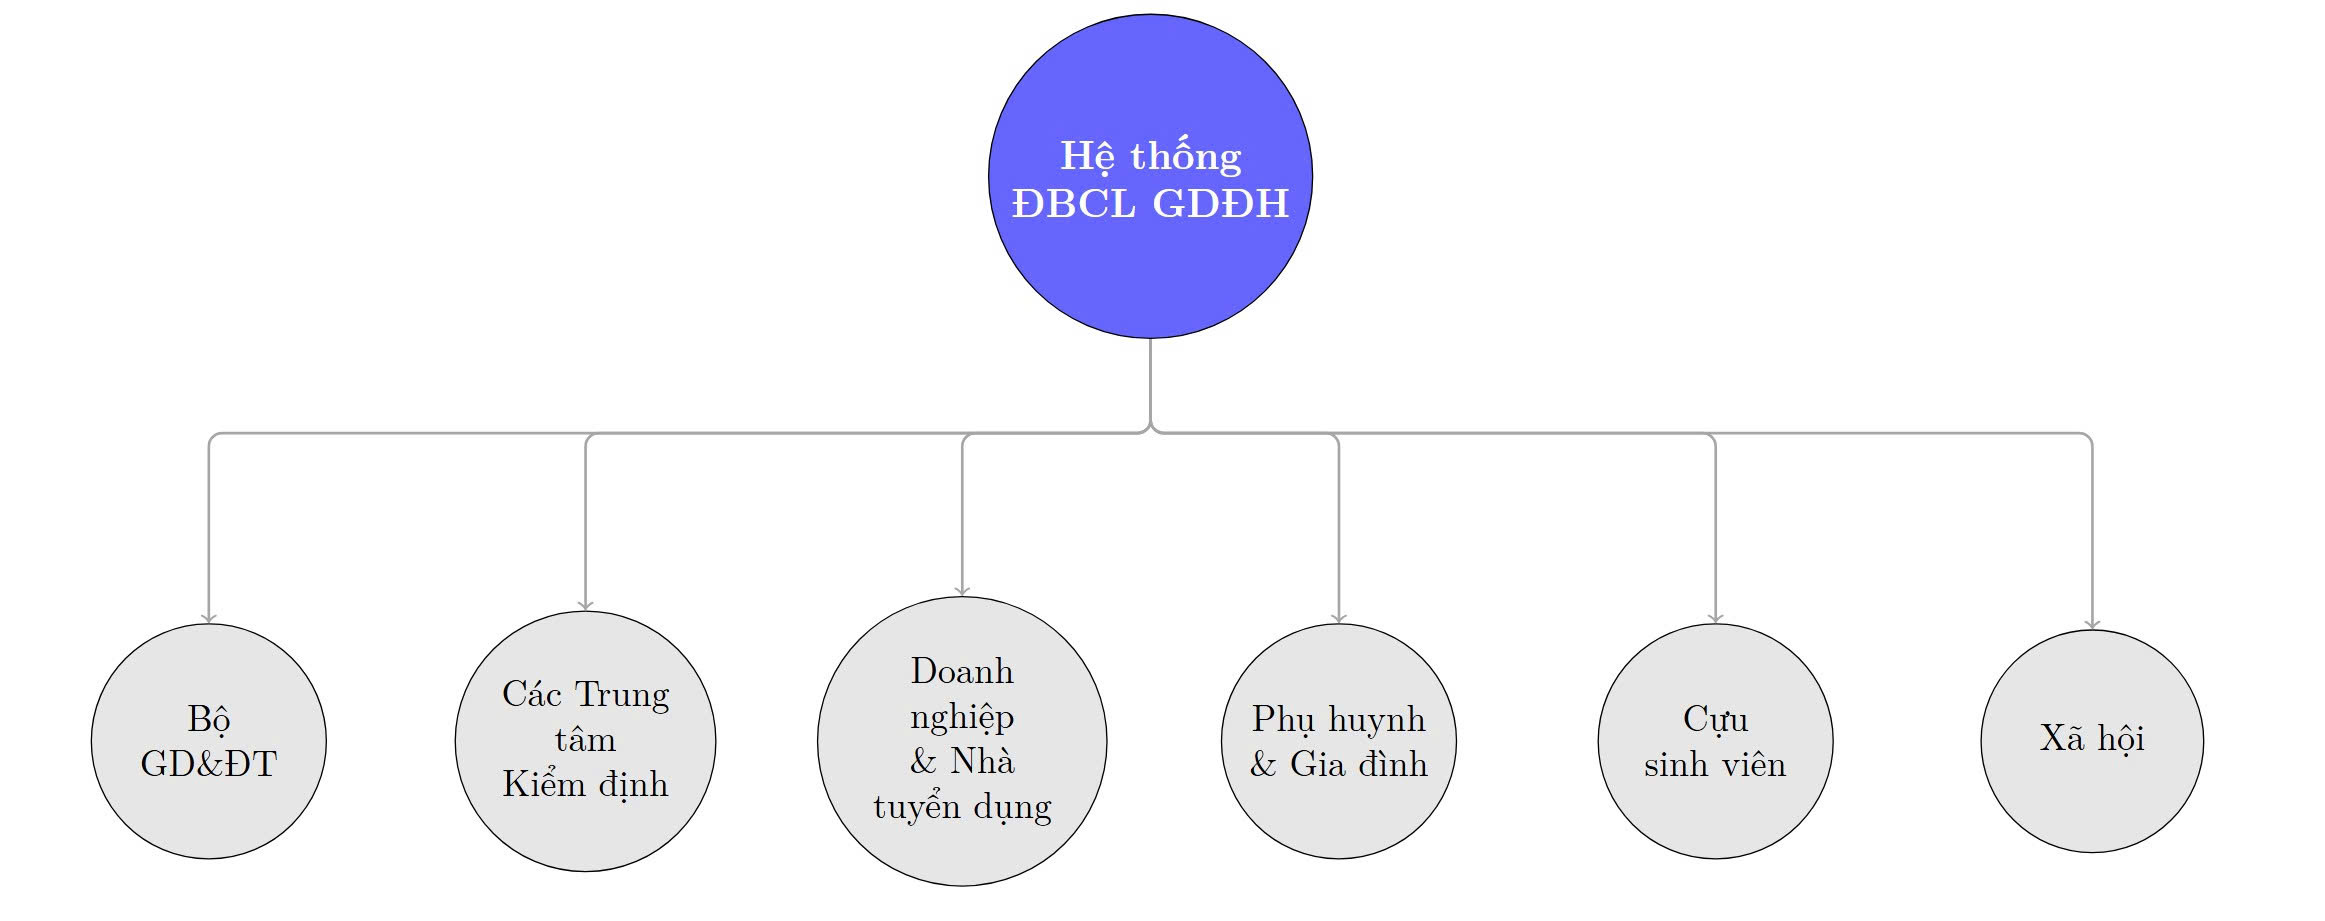
\includegraphics[width=\textwidth]{image/stakeholder_map.jpg} 
    \caption{越南高等教育质量保障体系中的利益相关者地图}
    \label{fig:stakeholder-map}
\end{figure}

\begin{itemize}
    \item \textbf{内部利益相关者 (Internal Stakeholders):}
        \begin{itemize}
            \item \textit{学校领导层(校董会、校领导班子):} 主要利益是学校的声誉、财务稳定、达成KPI指标以及遵守上级规定。
            \item \textit{教师与研究人员:} 利益包括学术自由、良好的工作条件、专业发展机会以及减少行政负担。
            \item \textit{行政人员(包括质量保障处干部):} 利益是流程清晰、有足够资源完成工作以及得到其他部门的合作。
            \item \textit{学生:} 核心利益是培养方案的质量、有效的教学方法、良好的学习环境、毕业后的就业机会以及合理的学费。
        \end{itemize}
    \item \textbf{外部利益相关者 (External Stakeholders):}
        \begin{itemize}
            \item \textit{教育培训部:} 利益是确保高等教育体系稳定运行、质量均衡,满足国家经济社会发展目标,并向政府和社会履行问责。
            \item \textit{教育质量认证中心:} 利益是维持其组织的声誉、专业性和独立性;完成被赋予的认证任务。
            \item \textit{企业与雇主:} 利益是能够招聘到具备与工作要求直接匹配的技能和知识的人力资源,减少再培训成本。
            \item \textit{家长与家庭:} 利益是为子女的投资(时间、金钱)带来应有的回报(孩子有好工作、成才)。
            \item \textit{校友:} 利益是学位证书的价值和母校声誉的提升,从而在职业网络中产生自豪感和机会。
            \item \textit{社会:} 利益是高等教育有助于创造一个公平、进步的社会,提供高质量的人力资源并维护文化价值观。
        \end{itemize}
\end{itemize}
该地图显示,质量保障体系必须服务于一个极其多样化的利益网络。一个质量改进的决策,例如增加学生的实践要求,可能会受到企业的欢迎,但却可能遭到教师(因工作量增加)或财务部门(因成本增加)的反对。识别和分析这些潜在的利益冲突,是构建一个有效的质量保障体系的第一步。



% done chuong 2 goi 2


% ======================================================================
% TRANG 11-13: THUYẾT CÁC BÊN LIÊN QUAN (PHẦN 2)
% ======================================================================

\subsubsection{利益相关者的显著性 (Stakeholder Salience)}

识别利益相关者仅仅是第一步。治理中的一个巨大挑战是如何处理来自这些群体的多样且常常相互矛盾的要求。并非所有利益相关者都具有同等的影响力。Mitchell, Agle和Wood(1997)提出了一个极具影响力的模型,用以确定利益相关者的“显著性”(salience),该模型基于三个核心属性\footcite{Mitchell1997}:

\begin{enumerate}
    \item \textbf{权力 (Power):} 利益相关者将其意志强加于组织之上的能力,迫使组织去做那些若无此压力则不会做的事情。权力可以来自对关键资源(如预算)的控制、颁布法规的能力或影响媒体的能力。
    \item \textbf{合法性 (Legitimacy):} 社会承认某一利益相关者的要求或行动在特定社会背景下是正当、适宜和正确的。合法性来自法律规定、合同或社会道德规范。
    \item \textbf{紧迫性 (Urgency):} 利益相关者的要求需要立即关注的程度。紧迫性取决于两个因素:时间敏感性(若不及时处理,要求将失去价值)和该要求对利益相关者的重要程度。
\end{enumerate}

根据拥有一、二或全部三个属性,利益相关者可被划分为不同优先级的群体,从“潜在”群体(latent stakeholders,仅有1个属性)到需要领导层最多关注的“决定性”群体(definitive stakeholders,拥有全部3个属性)。

将此模型应用于越南高等教育的质量保障体系,我们可以解释一些重要现象:
\begin{itemize}
    \item \textbf{教育培训部}是一个“决定性”利益相关者。该部拥有\textit{权力}(通过分配预算、颁发许可),拥有\textit{合法性}(依据《高等教育法》),并且其要求通常具有\textit{紧迫性}(与认证、报告周期挂钩)。因此,该部的声音分量最重,各大学通常优先满足其要求。
    \item \textbf{企业/雇主}是一个拥有\textit{合法性}(他们有权要求高质量的人力资源)和\textit{紧迫性}(人力需求不断变化)的利益相关者,但却缺乏直接\textit{权力}来迫使大学立即改变培养方案。这解释了为什么尽管企业不断抱怨学生质量,但大学培养方案的变革仍然缓慢。
    \item \textbf{学生和家长}拥有很高的\textit{合法性}和\textit{紧迫性},但他们的权力是分散的。只有当他们的要求通过大规模调查或媒体汇集起来时,他们的权力才会变得更加显著。
\end{itemize}
因此,显著性模型帮助我们理解,质量保障过程并非一个所有声音都平等的绝对民主过程,而是一个“政治舞台”,各大学必须不断权衡并优先考虑来自最具影响力的利益相关者的要求。

\subsubsection{利益相关者理论的应用与批判}

利益相关者理论提供了一个有效的分析工具,用以解读质量保障体系中的利益冲突。它有助于回答“质量为谁服务?”这一问题。通过识别利益相关者并分析其优先级,我们可以理解为什么质量的某些方面(例如:国际论文发表数量)会比其他方面(例如:学生的实践技能)更受重视。

然而,该理论也有其局限性。应用它时最大的挑战在于,当利益相互冲突时,如何找到一个最优方案来\textbf{平衡}这些利益。例如,为满足企业要求而加强实践教学会增加培养成本,可能导致学费上涨,从而引起学生和家长的反对。利益相关者理论很好地描述了这场争论,但并未提供解决它的明确公式。此外,该理论侧重于有形的关系和利益,但较少关注对组织行为有强大影响的无形文化规则和规范——而这正是新制度主义理论的长处。要理解具体的问责机制,我们需要借助第三种理论。

\subsection{委托代理理论 (Principal-Agent Theory)}
\label{subsec:uy_nhiem_nen_tang}

\subsubsection{起源与核心概念}
委托代理理论起源于经济学,特别是金融经济学和公司理论,其基础性工作由Stephen Ross等学者,特别是Michael Jensen和William Meckling在1970年代完成\footcite{JensenMeckling1976}。该理论旨在分析在一方(委托人 - Principal)雇佣或委托另一方(代理人 - Agent)代其执行某项工作时所产生的问题。

这种关系的核心问题(代理问题)源于两个基本条件:
\begin{enumerate}
    \item \textbf{目标冲突 (Conflict of Interest):} 委托人和代理人的利益并非总是一致。例如,股东(委托人)希望最大化利润,而管理者(代理人)可能希望最大化权力或其他个人利益。
    \item \textbf{信息不对称 (Information Asymmetry):} 代理人通常比委托人拥有更多关于工作及自身努力的信息。委托人难以完美地监督代理人的每一个行动。
\end{enumerate}
这两个条件的结合产生了两种主要风险\footcite{Eisenhardt1989}:
\begin{itemize}
    \item \textbf{道德风险 (Moral Hazard):} 合同签订后,由于委托人无法观察其努力程度,代理人可能不会尽全力工作。例如,一所大学(代理人)在从政府(委托人)获得预算后,可能不会尽最大努力投入于改进教学质量。
    \item \textbf{逆向选择 (Adverse Selection):} 签订合同前,代理人可能隐瞒信息或歪曲自身能力以求被选中。例如,一所大学可能会“美化”其自评报告,以获得认证机构的承认。
\end{itemize}
为解决这些问题,该理论提出了设计有效合同、创建激励机制(incentives)以协调利益等解决方案,最重要的是,建立\textbf{监督与报告系统(monitoring and reporting systems)}以减少信息不对称。


% done chuong 2 goi 3


% ======================================================================
% TRANG 16-18: THUYẾT ỦY NHIỆM (PHẦN 2) VÀ PHÊ PHÁN
% ======================================================================

\subsubsection{作为监督和合同机制的质量保障体系}

从委托代理理论的视角来看,整个外部质量保障体系可以被视为一个复杂的监督和合同机制,旨在解决“代理问题”。

\paragraph{多层次的委托代理关系:}
在高等教育中,关系不仅仅是单个委托人与代理人之间的关系。它是一系列相互嵌套的委托代理关系链,使得管理和监督变得复杂\footcite{Borgos2013}。我们可以将越南的这一关系链想象如下:
\begin{itemize}
    \item \textbf{第一层(政府 $\rightarrow$ 教育培训部):} 政府(委托人)将管理和发展国家高等教育体系的任务交给教育培训部(代理人)。
    \item \textbf{第二层(教育培训部 $\rightarrow$ 大学):} 教育培训部(委托人)向各大学(代理人)颁发办学许可并分配预算,期望各大学能够培养出高质量的人力资源并执行服务社会的研究任务。
    \item \textbf{第三层(校领导班子 $\rightarrow$ 院/系):} 校领导班子(委托人)将招生指标和预算分配给各院系(代理人),要求各院系保证其单位的培养和研究质量。
    \item \textbf{第四层(院/系 $\rightarrow$ 教师):} 院长/系主任(委托人)将教学任务分配给每位教师(代理人),并期望他们能以最佳方式完成授课。
\end{itemize}
这一委托代理链的存在解释了为什么来自最高层(政府)的要求在传达到下层时常常会被“干扰”或变形。

\paragraph{质量保障实践中的监督机制:}
为了在上述关系链中最大限度地减少道德风险和逆向选择,质量保障体系发展出了多种具体的监督机制:
\begin{itemize}
    \item \textbf{报告系统 (Reporting Systems):} 自评报告、年度报告、数据统计等要求,正是上级委托人收集下级代理人活动信息的工具。
    \item \textbf{外部认证 (External Accreditation):} 这是一种专门且正式的监督形式。认证机构(如VNU-CEA或AUN-QA)扮演着第三方“审计员”的角色,受委托人(教育培训部)信任,以核实信息并评估各大学(代理人)的活动\footcite{Borgos2013}。这一过程显著减少了信息不对称。
    \item \textbf{基于成果的合同 (Outcome-based Contracts):} 尽管在越南尚不普遍,但世界范围内的趋势是将预算分配与具体的产出结果(例如:学生就业率、国际发表数量)挂钩。这是一种旨在协调委托人与代理人利益的合同形式。
    \item \textbf{声誉建设 (Reputation Building):} 排名系统和公开认证结果也是一种监督机制。一所学校(代理人)的声誉成为一项重要资产,为了保护这项资产,他们有动力按照各委托人(学生、社会)的期望行事。
\end{itemize}

\subsubsection{委托代理理论的应用与批判}

委托代理理论提供了一套锐利的分析工具,用以剖析质量保障体系中的问责结构和监督机制。它逻辑地解释了为何需要报告、检查、定期认证等流程。特别是在分析合同性关系,如国家与被赋予自主权的公立大学之间的关系时,它尤其有用。

然而,机械地将委托代理理论应用于高等教育领域也有其显著的局限性\footcite{RIHE2022}:
\begin{itemize}
    \item \textbf{过分简化目标:} 该理论假设委托人的目标可以被明确定义。但在高等教育中,“质量”是一个多维度且难以衡量的概念。政府的目标可能是发展经济,而社会的目标是公平,学术界的目标则是创作自由。谁才是真正的“委托人”?
    \item \textbf{忽略文化与规范因素:} 该理论认为主体之间的关系主要基于经济利益和理性计算。它无法解释信任、共同价值观以及职业规范(例如:教师道德)在调节教师和学校行为中的作用。
    \item \textbf{难以应用完美的合同:} 在现实中,很难设计一个能预见所有情况并准确衡量代理人所有努力的合同。教育的“产品”(人)是极其复杂的,不能像工业产品那样容易衡量。
\end{itemize}
正因为这些局限性,分析质量保障体系不能仅仅依赖委托代理理论。必须将其与新制度主义理论(以理解无形规则)和利益相关者理论(以理解多样化利益)相结合,才能获得更全面、更准确的图景。

% ======================================================================
% TRANG 19-20: CÁC MÔ HÌNH ĐBCL HIỆN ĐẠI
% ======================================================================
\section{世界现代质量保障模型}
\label{sec:mo_hinh_hien_dai_the_gioi}

治理理论的发展和实践中的挑战,推动了日益精密的质量保障模型的诞生。这些模型不再固守单一理论,而是对传统方法的局限性进行综合和超越的努力。其中,混合模型和适应性框架这两个突出的趋势,对越南具有重要的参考意义\footcite{HybridModel2023}\footcite{AdaptiveQA2022}。

\subsection{混合模型 (Hybrid Model): 协调问责与改进}

\subsubsection{诞生背景与理念}
传统的质量保障体系通常陷入两个极端之一。一是,体系过分注重对外部的\textbf{问责制(accountability)}(自上而下),导致学校只专注于形式上、应付性地遵守规定,形成一种“合规文化”(culture of compliance)而非实质性改进。这是一种接近委托代理理论思维的模式。二是,体系过分注重\textbf{内部改进(improvement)}(自下而上),将全部权力交给单位自行评估,导致缺乏共同标准且难以确保对社会的问责。

混合模型应运而生,旨在解决这种紧张关系\footcite{EUA_Integration}。其理念是承认并整合这两个目标。它认为一个可持续的质量保障体系必须既能满足外部的控制和透明度要求,又能激发内部的改进动力和发展质量文化。混合模型不将问责与改进视为对立的目标,而是视其为一枚硬币的两面,相辅相成。例如,外部透明的问责要求可以为推动内部改进努力提供必要的数据和压力。反之,强大的内部改进文化将使学校更容易满足并超越外部的问责要求。

\subsubsection{组成部分与特点}
一个典型的混合模型通常具有以下特点:
\begin{itemize}
    \item \textbf{双重标准框架:} 体系可能包括一套用于问责目的的强制性\textbf{最低标准(minimum standards)},以及一套用于改进目的的鼓励性\textbf{提升标准(enhancement standards)}。
    \item \textbf{嵌套流程:} 外部认证活动的设计不仅旨在检查合规性,还旨在提供建设性建议,支持学校的改进过程。反之,内部自评和改进活动的结果被用作外部认证轮次中的重要证据。
    \item \textbf{质量保障机构的灵活角色:} 外部质量保障机构不仅扮演“裁判员”的角色,还扮演“伙伴”、“顾问”的角色,在改进过程中为学校提供支持。
\end{itemize}
欧洲质量保障体系的经验,尤其是在博洛尼亚进程之后,显示出向混合模型转变的明显趋势,其中认证流程越来越被设计为服务于质量提升的目标(enhancement-led accreditation)\footcite{EUA_Integration}。越南的实践,既要满足教育培训部的国家标准,又要参与如AUN-QA等区域认证项目,也正显示出一种混合模型正在逐渐形成的迹象,尽管可能尚非完全自觉\footcite{VNU-CEA2023}\footcite{HangNguyen2017}。

% done chuong 2 goi 4



% ======================================================================
% TRANG 21-22: KHUNG THÍCH ỨNG
% ======================================================================

\subsection{适应性框架 (Adaptive Framework): 在变化世界中的质量管理}
\label{subsec:khung_thich_ung}

\subsubsection{与传统方法的比较}
如果说混合模型解决了质量保障\textit{目标}的矛盾,那么适应性框架则解决了在不稳定和复杂环境中\textit{实施流程}的问题。传统的项目管理方法,通常被称为“瀑布模型”(Waterfall Model),遵循一个严格的线性序列:规划 → 设计 → 执行 → 测试 → 交付。该模型假设所有要求和条件都可以从一开始就明确确定,并且在整个过程中环境不会改变。

然而,在高等教育的现实中,尤其是在越南,情况则完全不同。教育部的政策可能改变,劳动力市场的需求波动,教育技术发展迅速,学校的资源也不稳定。采用一个僵化的、长达5年的瀑布式质量保障计划,通常会导致计划在尚未执行完毕时就已经过时。

适应性框架(Adaptive Framework),其源于敏捷软件开发(Agile)领域,正是为了解决这些问题而生\footcite{Wysocki2009}。它不是试图从一开始就制定一个完美的计划,而是将项目分解为短期的、重复的周期。在每个周期结束时,项目团队将重新评估结果,收集反馈,并为下一个周期调整计划。

\subsubsection{适应性框架的核心原则}
一个具有适应性的质量保障框架将基于以下原则运作:
\begin{itemize}
    \item \textbf{迭代学习 (Iterative Learning):} 整个质量保障流程被视为一个学习过程。学校可以不必每5年进行一次大型评估,而是可以针对具体方面(如教学方法、学生服务)进行更小规模的评估周期(例如,每年一次)。每个周期的结果将为改进下一个周期提供信息。
    \item \textbf{反馈循环 (Feedback Loops):} 该框架创建了快速且频繁的反馈循环。学校不必等到5年周期结束才有认证报告,而是可以在每学期或每学年后与学生、教师和企业组织反馈会议。
    \item \textbf{增量发展 (Incremental Development):} 质量改进不必同时进行,而是可以分阶段、逐步实施。例如,第一年,学校可以集中改进学生意见收集系统;第二年,专注于创新学习成果评估方法。
    \item \textbf{价值驱动的优先级排序 (Value-driven Prioritization):} 在每个周期,改进活动将根据其在当时为最重要利益相关者带来的价值来进行优先排序。
\end{itemize}

\subsubsection{对越南国情的适用性}
认为适应性框架特别适合越南国情的论点基于以下原因:
\begin{itemize}
    \item \textbf{动态的政策环境:} 越南关于高等教育的法规和政策可能会迅速变化。一个适应性框架允许学校灵活调整其质量保障策略,以适应新的要求,而无需推翻整个旧计划。
    \item \textbf{资源限制:} 学校不必投入巨额资金进行全面改革,而是可以根据其在每个阶段的有限资源,进行小规模、渐进式的改进。
    \item \textbf{逐步建立能力:} 立即实施一个复杂的质量保障体系可能会给人力团队带来过重负担。适应性框架允许学校边做边学,逐步且可持续地建立质量保障能力。
\end{itemize}
因此,将混合模型的理念与适应性框架的流程相结合,将创造出一种在目标上全面、在实施方式上灵活且务实的质量保障方法。这正是为越南构建建议模型的基础。

% ======================================================================
% TRANG 23-25: ĐỀ XUẤT MÔ HÌNH V-AQA
% ======================================================================
\section{为越南高等教育提出分析模型:混合与适应性模型 (V-AQA)}
\label{sec:mo_hinh_V-AQA_de_xuat}

\subsection{建立一个综合模型的必要性论证}
\label{subsec:luan_giai_V-AQA}
通过以上各部分的分析可以看出,使用单一理论来分析越南高等教育的质量保障体系是不全面的,并可能导致片面的结论。
\begin{itemize}
    \item \textbf{如果仅使用新制度主义},我们将能解释为何各学校会形式化地遵守规定,但难以解释来自内部的实质性改进努力或利益冲突。
    \item \textbf{如果仅使用利益相关者理论},我们将能看到利益多样化的图景,但却缺乏分析工具来解释为何某些方面的声音比其他方面更有分量,也无法解释报告和监督机制。
    \item \textbf{如果仅使用委托代理理论},我们将能清晰理解问责结构,但却会忽略文化、规范因素以及无法简化为单纯合同的复杂合作关系。
\end{itemize}

因此,越南的国情需要一个综合的分析框架,一个能够融合不同视角的模型。本论文提出了这样一个模型,名为\textbf{越南高等教育混合与适应性质量保障模型(The Vietnam - Adaptive Quality Assurance Model,简称 V-AQA)}。

该模型具有\textbf{混合性(Hybrid)},因为它承认并试图协调两个并行且时而矛盾的目标:
\begin{enumerate}
    \item \textbf{对外部的问责制(External Accountability):} 满足教育培训部、认证机构和社会的要求,以获得合法性和资源(反映了新制度主义和委托代理理论的视角)。
    \item \textbf{来自内部的改进(Internal Improvement):} 为内部利益相关者(学生、教师)创造价值,并推动一种内生的质量文化(反映了利益相关者理论的视角)。
\end{enumerate}

同时,该模型具有\textbf{适应性(Adaptive)},因为它在实施过程中强调灵活性,允许大学根据反馈和环境变化,以短期周期调整其质量保障活动,而不是遵循一个僵化的五年计划。

\subsection{V-AQA模型的结构与核心要素}
\label{subsec:cau_truc_V-AQA}

V-AQA模型的结构如同一座神殿,以理论为基石,以最终目标为屋顶,并由五个核心要素作为五根支柱支撑。这五个要素并非独立运作,而是相互作用、相互巩固,形成一个稳固的系统(见图 \ref{fig:v-aqa-model-detailed})。

\begin{figure}[h!]
    \centering
    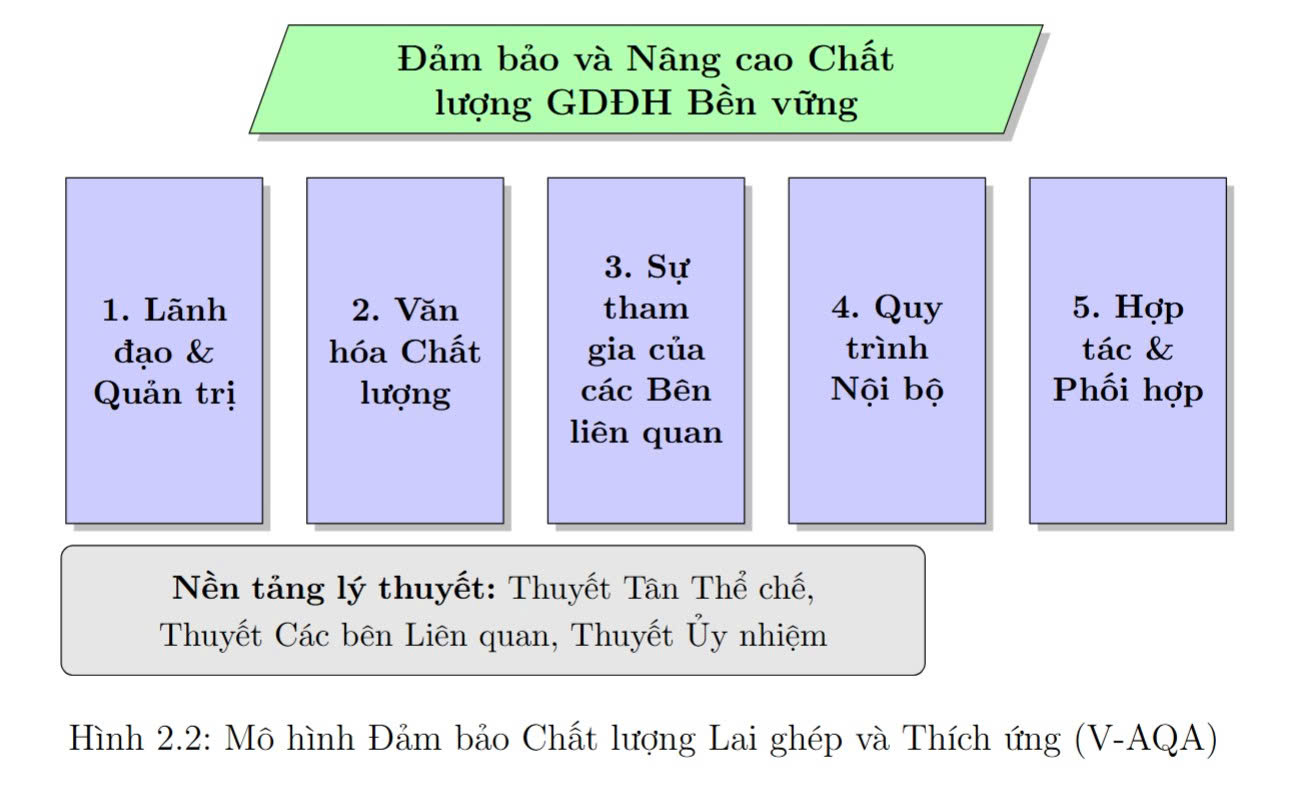
\includegraphics[width=0.9\textwidth]{image/mo_hinh_V-AQA.jpg}
    \caption{混合与适应性质量保障模型 (V-AQA)}
    \label{fig:v-aqa-model-detailed}
\end{figure}

\subsubsection{要素1的详细分析:领导与治理 (Leadership \& Governance)}
\label{subsubsec:thanh_to_1}

\paragraph{定义与范围:}
领导与治理要素是整个质量保障体系的源头,为之指明方向并提供资源。它不仅是行政管理活动,更是领导层在构建愿景、激发灵感以及建立有效治理结构以实现该愿景的能力。在越南的背景下,该要素包括校董会、校领导班子以及各级院、处、室领导的作用。它通过颁布关于质量的战略、政策及执行这些政策的承诺来体现。

\paragraph{理论与实践基础:}
该要素受到\textbf{委托代理理论}和\textbf{新制度主义理论}的强烈映射。
\begin{itemize}
    \item 从委托代理理论的角度看,学校领导层既是上级管理机构(教育培训部)的\textit{代理人},有责任执行国家政策;又是下级单位(院、系)的\textit{委托人},有责任监督并确保这些单位有效运作。明确的治理结构和责任划分是解决内部代理问题的先决条件。
    \item 从新制度主义的角度看,领导者是“解读”并诠释来自制度场域压力的角色。他们决定学校的战略:是被动遵守、模仿成功模式,还是主动寻求独特道路以创造差异化和独特的合法性。领导者的愿景将塑造学校与外部环境互动的方式。
\end{itemize}

\paragraph{实践中的指标与表现:}
为了评估一所大学在该要素上的发展水平,可以考察以下指标:
\begin{itemize}
    \item 是否存在一份详细的校级\textit{质量战略},并将其融入学校的总体发展战略中。
    \item 校领导班子、校董会涉及质量保障问题的会议频率和内容。
    \item 为质量保障活动分配资源(财务、人力)的程度。
    \item 规定质量保障相关单位职能、任务的文件的明确性。
    \item 关于干部、教师对领导层在质量工作中的承诺和导向作用的意见调查结果。
\end{itemize}
对这些指标的分析将在本论文的现状章节中详细进行。

% done chuong 2 goi 5


% ======================================================================
% TRANG 26-28: PHÂN TÍCH CHI TIẾT THÀNH TỐ 2: VĂN HÓA CHẤT LƯỢNG
% ======================================================================

\subsubsection{要素2的详细分析:质量文化 (Quality Culture)}
\label{subsubsec:thanh_to_2}

\paragraph{定义与范围:}
质量文化不仅是对质量的认知或口号,而是一个共享的价值观、信念、期望和承诺的集合,它塑造了一个教育机构中所有成员在保障和提升质量方面的行为\footcite{HarveyStensaker}。它是在谈论质量时“我们在这里做事的方式”(the way we do things around here)。该要素与“合规文化”(culture of compliance)相对立,在合规文化中,质量保障活动只是为了应付外部要求而机械地执行。

质量文化的范围非常广泛,它渗透到学术生活的每一个角落,从一名教师如何准备教案,一个院系如何组织专业研讨会,到学校领导层如何做出战略决策。一个强大的质量文化将把质量保障从一种行政负担转变为个人和组织发展的内在动力。

\paragraph{理论基础与质量文化的维度:}
质量文化通过\textbf{新制度主义理论}的视角得到最清晰的体现,特别是其\textit{规范性(normative)}和\textit{文化-认知性(cultural-cognitive)}两大支柱。
\begin{itemize}
    \item \textbf{规范性方面:} 质量文化通过职业规范形成和巩固。当“持续改进”或“以学习者为中心”成为学术界所重视的规范时,个人为了被视为专业的教育者和管理者,会倾向于按照该规范行事。
    \item \textbf{文化-认知性方面:} 质量文化作为一种无需思考即被接受的脚本或常识而存在。届时,收集学生反馈或定期审查培养方案不再是一项要求,而是一件“理所当然”必须做的事情。
\end{itemize}

为了系统地分析质量文化,可以使用Harvey和Stensaker(2008)的模型,该模型将质量文化分为四种类型,反映了组织的成熟度\footcite{HarveyStensaker}:
\begin{enumerate}
    \item \textbf{反应型文化 (Reactive Culture):} 组织仅在出现问题或有外部检查要求时才关注质量。这是最低的层次。
    \item \textbf{响应型文化 (Responsive Culture):} 组织开始建立流程和体系以响应质量要求,但动力主要仍来自外部。许多越南大学目前正处于此阶段,为应对认证评估而建立质量保障部门和流程。
    \item \textbf{再生/改进型文化 (Regenerative Culture):} 这是一个质的飞跃。组织有能力自我评估,自我发现问题,并主动实施持续改进的循环。改进的动力来自内部。
    \item \textbf{繁殖/传播型文化 (Reproductive Culture):} 在最高层次,组织不仅自我改进,还成为典范,向外传播关于质量的最佳实践,为其他组织塑造规范。
\end{enumerate}
该模型为诊断和确定一所大学质量文化的发展目标提供了有用的工具。

\paragraph{在越南实践中的指标与表现:}
质量文化是一个抽象的概念,但可以通过具体的指标和表现来间接衡量:
\begin{itemize}
    \item \textbf{领导层的承诺:} 公开发言、战略文件以及资源分配是否显示出质量保障是真正的优先事项。
    \item \textbf{教师和员工的态度:} 关于工作满意度、对质量保障活动(视其为负担还是机遇)的态度的调查结果,以及自愿参与改进活动的程度。
    \item \textbf{内部使用的语言:} 内部文件和会议是使用“遵守”、“响应要求”的语言,还是“提升”、“改进”、“卓越”的语言?
    \item \textbf{认可与奖励机制:} 学校是否有机制来表彰和奖励有质量改进创举的个人和单位?
\end{itemize}
正如专家报告所反映的,越南的现状表明,许多大学仍在努力从“响应型”文化向“改进型”文化转型。来自认证评估的压力通常会产生临时性的活动,质量文化尚未真正深入到每位教师的日常工作中\footcite{ExpertPerspectivesVN}\footcite{CommonFailureCriteria}。这是V-AQA模型需要解决的最大挑战之一。

% ======================================================================
% TRANG 29-30: PHÂN TÍCH CHI TIẾT THÀNH TỐ 3: SỰ THAM GIA CỦA CÁC BÊN LIÊN QUAN
% ======================================================================

\subsubsection{要素3的详细分析:利益相关者的参与 (Stakeholder Engagement)}
\label{subsubsec:thanh_to_3}

\paragraph{定义与范围:}
利益相关者的参与不仅仅是“征求意见”或“举办研讨会”。它是一个有系统的、有目的的过程,旨在将利益相关者吸引到质量保障的各个环节中,从培养方案的设计,到教与学的过程,再到评估和改进。这是“质量为谁服务?”这一理念的实现,承认一个高质量的培养方案必须为不同的对象群体创造价值。

参与的范围很广,包括从低到高的多种形式:
\begin{itemize}
    \item \textbf{告知 (Informing):} 向利益相关者单向提供信息。
    \item \textbf{咨询 (Consulting):} 征求利益相关者的意见和反馈。
    \item \textbf{卷入 (Involving):} 在整个过程中与利益相关者直接合作。
    \item \textbf{协作 (Collaborating):} 在决策中成为合作伙伴。
    \item \textbf{授权 (Empowering):} 将最终决策权交给利益相关者。
\end{itemize}
一个成熟的质量保障体系需要根据具体问题和具体利益相关者,为不同层次的参与提供机制\footcite{Arnstein1969}。

\paragraph{理论与实践基础:}
该要素是\textbf{利益相关者理论}的直接应用。它将重心从一个封闭、内向的管理模式转向一个开放、外向的模式。这也是混合模型的一个核心要素,因为正是来自外部利益相关者的反馈和要求,构成了内部改进活动的重要动力。

国际实践,特别是欧洲的经验表明,利益相关者,尤其是学生和雇主的参与,是现代质量保障体系中不可或`缺的要素。像AUN-QA这样的标准体系也对在审查和改进培养方案中收集和使用利益相关者反馈提出了明确要求\footcite{ENQA_Stakeholder2018}\footcite{AUN-QAGuide}。

\paragraph{在越南实践中的指标与表现:}
该要素的发展水平可以通过以下指标进行评估:
\begin{itemize}
    \item \textbf{有外部人员参与的委员会的存在:} 例如,科学与培养委员会、每个专业的行业咨询委员会(Industry Advisory Board)。
    \item \textbf{咨询活动的频率和实质性:} 与雇主举行的研讨会数量、校友调查、为学生设立的反馈渠道。
    \item \textbf{影响的证据:} 是否有具体证据表明培养方案已根据企业或校友的反馈进行了调整和更新。
    \item \textbf{学生在各委员会中的角色:} 学生在院级、校级委员会中是否有代表,他们的声音是否得到实质性的倾听和记录。
\end{itemize}
在越南,这是仍存在诸多局限的要素之一。报告通常指出,校企联系仍然松散且形式化。培养方案的制定通常主要基于学术团队的观点,而很少有雇主的实质性参与\footcite{CommonFailureCriteria}。因此,加强利益相关者的参与是越南高等教育质量保障体系改革的一个重要方向。

% done chuong 2 goi 6


% ======================================================================
% TRANG 31-35: PHÂN TÍCH CHI TIẾT THÀNH TỐ 4: QUY TRÌNH NỘI BỘ
% ======================================================================

\subsubsection{要素4的详细分析:内部流程 (Internal Processes)}
\label{subsubsec:thanh_to_4}

\paragraph{定义与范围:}
如果说前面的要素关注的是“为什么”(理论)、“谁”(领导者、利益相关者)和“什么”(文化),那么要素4则关注\textbf{“如何做?”}的问题。内部流程是一所教育机构用来系统地管理核心学术活动以保障和提升质量的一整套标准化的政策、程序、指南和工具。

这是质量保障体系的“运行机器”,将质量战略和目标转化为具体且可衡量的行动。该要素的范围涵盖了学生的整个学术生命周期,从培养方案的设计到学生毕业并由雇主评估。在本论文的框架内,我们将重点关注三个最重要的子流程:(1)培养方案(CDĐT)的设计与审查;(2)教-学活动与评估的管理;以及(3)数据收集与分析系统。

\paragraph{子流程4.1:培养方案(CDĐT)的设计与审查}
这是决定学校所提供的教育“产品”的基础流程。一个有效的流程必须确保培养方案既具科学性,又能满足利益相关者的需求。

\textit{理论基础:} 该流程是三大基础理论的交汇点。\textbf{利益相关者理论}要求流程必须有机制来收集和整合来自学生、企业的要求。\textbf{新制度主义理论}解释了为什么培养方案通常必须遵守教育培训部颁布的“课程框架”(强制性同形),并倾向于参考知名大学(模仿性同形)。\textbf{委托代理理论}将培养方案视为学校(代理人)承诺为社会和国家(委托人)执行的一种详细“合同”。

\textit{标准流程中的步骤:} 一个有效的培养方案设计与审查流程通常包括以下步骤,正如AUN-QA等国际标准所建议的\footcite{AUN-QAGuide}:
\begin{enumerate}
    \item \textbf{确定预期学习成果(Expected Learning Outcomes - ELOs):} 这是最重要的一步。ELOs必须基于与利益相关者(特别是雇主)的协商来制定,必须清晰、可衡量,并与学校的使命和愿景相符。
    \item \textbf{构建课程地图(Curriculum Mapping):} 设计课程和学习活动,使其能够逻辑地、系统地为实现既定的ELOs做出贡献。该技术有助于确保整个方案的一致性和建设性对齐(constructive alignment)。
    \item \textbf{审批与颁布:} 必须有一个科学与培养委员会(有外部专家参与)在正式颁布前对培养方案进行审定和批准。
    \item \textbf{定期审查与改进:} 必须有一个定期流程(例如:每2-3年一次),根据来自校友、雇主的反馈、学生的学习成果以及行业的新趋势来重新审查培养方案。
\end{enumerate}

\textit{越南现状:} 这是仍然存在许多薄弱环节的领域之一。认证报告通常指出,许多学校的培养方案设计流程仍然是封闭的,主要依赖于教师团队的经验,而缺乏企业的实质性参与。课程审查通常没有系统地进行,导致培养方案落后于劳动力市场的要求\footcite{CommonFailureCriteria}。

\paragraph{子流程4.2:教-学活动与评估的管理}
如果说培养方案是“设计图”,那么这就是“施工”过程。教-学活动和评估的质量直接决定了学生的学习体验和学习成果。

\textit{理论基础:} \textbf{委托代理理论}解释了监督教学活动(听课、检查)的必要性,以减少道德风险(教师备课不认真)。\textbf{利益相关者理论}强调了学生通过调查系统对教学质量提供反馈的作用。

\textit{流程的组成部分:}
\begin{itemize}
    \item \textbf{教学管理流程:} 包括关于制定详细课程大纲、准备教案、应用积极教学方法以及听课、向教师提建议的机制的规定。
    \item \textbf{学生学习成果评估流程:} 需要多样化评估形式,不仅仅依赖期末考试。过程性评估、项目、演讲、团队合作以及基于实践能力的测试等形式需要被标准化并广泛应用。必须有建立试题库、出题、阅卷和复核的透明、公平的流程。
    \item \textbf{反馈流程(Feedback):} 必须有机制让学生定期对每门课程和教师提出反馈。更重要的是,必须有流程来处理这些反馈,并向学生通报已进行的改变和改进。
\end{itemize}

\textit{越南现状:} 这也是一个固有的弱点。认证报告经常指出,单向讲授法被滥用,评估方法主要依赖记忆,以及来自学生的反馈系统仍然是形式化的,并未真正影响到教学的改进\footcite{ExpertPerspectivesVN}\footcite{CommonFailureCriteria}。

\paragraph{子流程4.3:数据收集与分析系统 – 基于证据的治理基础}

这是整个质量保障体系的“神经系统”,是支持其他流程的最重要的技术要素。没有它,所有改进决策都有可能变得主观和缺乏依据。

\textit{理论基础与作用:} 该系统是\textbf{委托代理理论}中监督机制的实现,是倾听\textbf{利益相关者}声音的工具,也是\textbf{新制度主义理论}下专业化、合理化的一个象征。它使学校能够从基于经验的管理模式转向基于证据的治理(evidence-based governance)。

\textit{核心功能:}
\begin{enumerate}
    \item \textbf{收集 (Collection):} 建立流程,从多个来源(学生学习成果、招生数据、教师人事信息、满意度调查结果、校友就业数据、财务数据等)一致地、定期地收集数据。
    \item \textbf{管理 (Management):} 构建一个集中的数据库(database)或数据仓库(data warehouse)来存储、清理和管理已收集的数据。
    \item \textbf{分析 (Analysis):} 使用统计和分析工具将原始数据转化为有意义的信息。例如:寻找教学方法与学生学习成果之间的相关性,或分析影响学生辍学率的因素。
    \item \textbf{报告与可视化 (Reporting \& Visualization):} 构建自动化的报告(reports)和仪表盘(dashboards)系统,直观地为不同级别的管理层提供信息,以支持决策。
\end{enumerate}

\textit{越南现状:} 这被认为是越南质量评估报告中最大和最普遍的挑战\footcite{CommonFailureCriteria}\footcite{AUN-QA_Challenges_VN}。学校通常缺乏一个集成的数据系统;数据分散在不同的部门,没有标准化,难以利用。决策通常仍然更多地依赖于领导的经验,而不是客观的数据分析。构建这样一个系统需要对技术和人力进行大量投资,这是一个巨大的障碍。

\paragraph{关于内部流程要素的结论:}
这三个子流程相互之间联系紧密。一个设计良好的培养方案(4.1)如果不能通过有效的教-学和评估方法(4.2)来实施,将毫无意义。而要知道流程(4.1)和(4.2)是否有效,学校需要一个强大的数据系统来衡量和分析(4.3)。任何一个流程的薄弱都会影响到整个系统。因此,标准化和改进这些内部流程是任何质量保障努力的核心任务。

% done chuong 2 goi 7




















	
    \bibliographystyle{gbt7714-numerical}
	\bibliography{ref/refs}
	
	\begin{appendix}
	% !Mode:: "TeX:UTF-8"

\chapter{外文资料原文}
\label{cha:engorg}
As one of the most widely used techniques in operations research, {\em
  mathematical programming} is defined as a means of maximizing a quantity known
as {\em objective function}, subject to a set of constraints represented by
equations and inequalities. Some known subtopics of mathematical programming are
linear programming, nonlinear programming, multiobjective programming, goal
programming, dynamic programming, and multilevel programming$^{[1]}$.

It is impossible to cover in a single chapter every concept of mathematical
programming. This chapter introduces only the basic concepts and techniques of
mathematical programming such that readers gain an understanding of them
throughout the book$^{[2,3]}$.


\section{Single-Objective Programming}
The general form of single-objective programming (SOP) is written
as follows,
\begin{equation}\tag*{(123)} % 如果附录中的公式不想让它出现在公式索引中,那就请
                             % 用 \tag*{xxxx}
\left\{\begin{array}{l}
\max \,\,f(x)\\[0.1 cm]
\mbox{subject to:} \\ [0.1 cm]
\qquad g_j(x)\le 0,\quad j=1,2,\cdots,p
\end{array}\right.
\end{equation}
which maximizes a real-valued function $f$ of
$x=(x_1,x_2,\cdots,x_n)$ subject to a set of constraints.

\newtheorem{mpdef}{Definition}[chapter]
\begin{mpdef}
In SOP, we call $x$ a decision vector, and
$x_1,x_2,\cdots,x_n$ decision variables. The function
$f$ is called the objective function. The set
\begin{equation}\tag*{(456)} % 这里同理,其它不再一一指定。
S=\left\{x\in\Re^n\bigm|g_j(x)\le 0,\,j=1,2,\cdots,p\right\}
\end{equation}
is called the feasible set. An element $x$ in $S$ is called a
feasible solution.
\end{mpdef}

\newtheorem{mpdefop}[mpdef]{Definition}
\begin{mpdefop}
A feasible solution $x^*$ is called the optimal
solution of SOP if and only if
\begin{equation}
f(x^*)\ge f(x)
\end{equation}
for any feasible solution $x$.
\end{mpdefop}

One of the outstanding contributions to mathematical programming was known as
the Kuhn-Tucker conditions\ref{eq:ktc}. In order to introduce them, let us give
some definitions. An inequality constraint $g_j(x)\le 0$ is said to be active at
a point $x^*$ if $g_j(x^*)=0$. A point $x^*$ satisfying $g_j(x^*)\le 0$ is said
to be regular if the gradient vectors $\nabla g_j(x)$ of all active constraints
are linearly independent.

Let $x^*$ be a regular point of the constraints of SOP and assume that all the
functions $f(x)$ and $g_j(x),j=1,2,\cdots,p$ are differentiable. If $x^*$ is a
local optimal solution, then there exist Lagrange multipliers
$\lambda_j,j=1,2,\cdots,p$ such that the following Kuhn-Tucker conditions hold,
\begin{equation}
\label{eq:ktc}
\left\{\begin{array}{l}
    \nabla f(x^*)-\sum\limits_{j=1}^p\lambda_j\nabla g_j(x^*)=0\\[0.3cm]
    \lambda_jg_j(x^*)=0,\quad j=1,2,\cdots,p\\[0.2cm]
    \lambda_j\ge 0,\quad j=1,2,\cdots,p.
\end{array}\right.
\end{equation}
If all the functions $f(x)$ and $g_j(x),j=1,2,\cdots,p$ are convex and
differentiable, and the point $x^*$ satisfies the Kuhn-Tucker conditions
(\ref{eq:ktc}), then it has been proved that the point $x^*$ is a global optimal
solution of SOP.

\subsection{Linear Programming} 
\label{sec:lp}

If the functions $f(x),g_j(x),j=1,2,\cdots,p$ are all linear, then SOP is called
a {\em linear programming}.

The feasible set of linear is always convex. A point $x$ is called an extreme
point of convex set $S$ if $x\in S$ and $x$ cannot be expressed as a convex
combination of two points in $S$. It has been shown that the optimal solution to
linear programming corresponds to an extreme point of its feasible set provided
that the feasible set $S$ is bounded. This fact is the basis of the {\em simplex
  algorithm} which was developed by Dantzig as a very efficient method for
solving linear programming.
\begin{table}[ht]
\centering
  \centering
  \caption*{Table~1\hskip1em This is an example for manually numbered table, which would not appear in the list of tables}
  \label{tab:badtabular2}
  \begin{tabular}[c]{|c|m{0.8in}|c|c|c|c|c|}\hline
    \multicolumn{2}{|c|}{Network Topology} & \# of nodes & 
    \multicolumn{3}{c|}{\# of clients} & Server \\\hline
    GT-ITM & Waxman Transit-Stub & 600 &
    \multirow{2}{2em}{2\%}& 
    \multirow{2}{2em}{10\%}& 
    \multirow{2}{2em}{50\%}& 
    \multirow{2}{1.2in}{Max. Connectivity}\\\cline{1-3}
    \multicolumn{2}{|c|}{Inet-2.1} & 6000 & & & &\\\hline
    \multirow{2}{1in}{Xue} & Rui  & Ni &\multicolumn{4}{c|}{\multirow{2}*{\bnuthesis}}\\\cline{2-3}
    & \multicolumn{2}{c|}{ABCDEF} &\multicolumn{4}{c|}{} \\\hline
\end{tabular}  
\end{table}

Roughly speaking, the simplex algorithm examines only the extreme points of the
feasible set, rather than all feasible points. At first, the simplex algorithm
selects an extreme point as the initial point. The successive extreme point is
selected so as to improve the objective function value. The procedure is
repeated until no improvement in objective function value can be made. The last
extreme point is the optimal solution.

\subsection{Nonlinear Programming}

If at least one of the functions $f(x),g_j(x),j=1,2,\cdots,p$ is nonlinear, then
SOP is called a {\em nonlinear programming}.

A large number of classical optimization methods have been developed to treat
special-structural nonlinear programming based on the mathematical theory
concerned with analyzing the structure of problems.

Now we consider a nonlinear programming which is confronted solely with
maximizing a real-valued function with domain $\Re^n$.  Whether derivatives are
available or not, the usual strategy is first to select a point in $\Re^n$ which
is thought to be the most likely place where the maximum exists. If there is no
information available on which to base such a selection, a point is chosen at
random. From this first point an attempt is made to construct a sequence of
points, each of which yields an improved objective function value over its
predecessor. The next point to be added to the sequence is chosen by analyzing
the behavior of the function at the previous points. This construction continues
until some termination criterion is met. Methods based upon this strategy are
called {\em ascent methods}, which can be classified as {\em direct methods},
{\em gradient methods}, and {\em Hessian methods} according to the information
about the behavior of objective function $f$. Direct methods require only that
the function can be evaluated at each point. Gradient methods require the
evaluation of first derivatives of $f$. Hessian methods require the evaluation
of second derivatives. In fact, there is no superior method for all
problems. The efficiency of a method is very much dependent upon the objective
function.


\chapter{外文资料的调研阅读报告或书面翻译}
\section{单目标规划}
北冥有鱼,其名为鲲。鲲之大,不知其几千里也。化而为鸟,其名为鹏。鹏之背,不知其几
千里也。怒而飞,其翼若垂天之云。是鸟也,海运则将徙于南冥。南冥者,天池也。 
\begin{equation}\tag*{(123)}
 p(y|\mathbf{x}) = \frac{p(\mathbf{x},y)}{p(\mathbf{x})}=
\frac{p(\mathbf{x}|y)p(y)}{p(\mathbf{x})}
\end{equation}

吾生也有涯,而知也无涯。以有涯随无涯,殆已!已而为知者,殆而已矣!为善无近名,为
恶无近刑,缘督以为经,可以保身,可以全生,可以养亲,可以尽年。

\subsection{线性规划}
庖丁为文惠君解牛,手之所触,肩之所倚,足之所履,膝之所倚,砉然响然,奏刀騞然,莫
不中音,合于桑林之舞,乃中经首之会。
\begin{table}[ht]
\centering
  \caption*{表~1\hskip1em 这是手动编号但不出现在索引中的一个表格例子}
  \label{tab:badtabular3}
  \begin{tabular}[c]{|c|m{0.8in}|c|c|c|c|c|}\hline
    \multicolumn{2}{|c|}{Network Topology} & \# of nodes & 
    \multicolumn{3}{c|}{\# of clients} & Server \\\hline
    GT-ITM & Waxman Transit-Stub & 600 &
    \multirow{2}{2em}{2\%}& 
    \multirow{2}{2em}{10\%}& 
    \multirow{2}{2em}{50\%}& 
    \multirow{2}{1.2in}{Max. Connectivity}\\\cline{1-3}
    \multicolumn{2}{|c|}{Inet-2.1} & 6000 & & & &\\\hline
    \multirow{2}{1in}{Xue} & Rui  & Ni &\multicolumn{4}{c|}{\multirow{2}*{\bnuthesis}}\\\cline{2-3}
    & \multicolumn{2}{c|}{ABCDEF} &\multicolumn{4}{c|}{} \\\hline
\end{tabular}  
\end{table}

\begin{table}[ht]
\centering
  \caption{正常附录表格的例子}
  \label{tab:badtabular3}
  \begin{tabular}[c]{|c|m{0.8in}|c|c|c|c|c|}\hline
    \multicolumn{2}{|c|}{Network Topology} & \# of nodes & 
    \multicolumn{3}{c|}{\# of clients} & Server \\\hline
    GT-ITM & Waxman Transit-Stub & 600 &
    \multirow{2}{2em}{2\%}& 
    \multirow{2}{2em}{10\%}& 
    \multirow{2}{2em}{50\%}& 
    \multirow{2}{1.2in}{Max. Connectivity}\\\cline{1-3}
    \multicolumn{2}{|c|}{Inet-2.1} & 6000 & & & &\\\hline
    \multirow{2}{1in}{Xue} & Rui  & Ni &\multicolumn{4}{c|}{\multirow{2}*{\bnuthesis}}\\\cline{2-3}
    & \multicolumn{2}{c|}{ABCDEF} &\multicolumn{4}{c|}{} \\\hline
\end{tabular}  
\end{table}

文惠君曰:“嘻,善哉!技盖至此乎?”庖丁释刀对曰:“臣之所好者道也,进乎技矣。始臣之
解牛之时,所见无非全牛者;三年之后,未尝见全牛也;方今之时,臣以神遇而不以目视,
官知止而神欲行。依乎天理,批大郤,导大窾,因其固然。技经肯綮之未尝,而况大坬乎!
良庖岁更刀,割也;族庖月更刀,折也;今臣之刀十九年矣,所解数千牛矣,而刀刃若新发
于硎。彼节者有间而刀刃者无厚,以无厚入有间,恢恢乎其于游刃必有余地矣。是以十九年
而刀刃若新发于硎。虽然,每至于族,吾见其难为,怵然为戒,视为止,行为迟,动刀甚微,
謋然已解,如土委地。提刀而立,为之而四顾,为之踌躇满志,善刀而藏之。”

文惠君曰:“善哉!吾闻庖丁之言,得养生焉。”


\subsection{非线性规划}
孔子与柳下季为友,柳下季之弟名曰盗跖。盗跖从卒九千人,横行天下,侵暴诸侯。穴室枢
户,驱人牛马,取人妇女。贪得忘亲,不顾父母兄弟,不祭先祖。所过之邑,大国守城,小
国入保,万民苦之。孔子谓柳下季曰:“夫为人父者,必能诏其子;为人兄者,必能教其弟。
若父不能诏其子,兄不能教其弟,则无贵父子兄弟之亲矣。今先生,世之才士也,弟为盗
跖,为天下害,而弗能教也,丘窃为先生羞之。丘请为先生往说之。”

柳下季曰:“先生言为人父者必能诏其子,为人兄者必能教其弟,若子不听父之诏,弟不受
兄之教,虽今先生之辩,将奈之何哉?且跖之为人也,心如涌泉,意如飘风,强足以距敌,
辩足以饰非。顺其心则喜,逆其心则怒,易辱人以言。先生必无往。”

孔子不听,颜回为驭,子贡为右,往见盗跖。


\chapter{其它附录}
前面两个附录主要是给本科生做例子。其它附录的内容可以放到这里,当然如果你愿意,可
以把这部分也放到独立的文件中,然后将其 \verb|\input| 到主文件中。
	\end{appendix}
	
	% !Mode:: "TeX:UTF-8"


\begin{paper}
\begin{enumerate}
	\item Yang Y, Ren T L, Zhang L T, et al. Miniature microphone with silicon-based ferroelectric thin films. Integrated Ferroelectrics, 2003, 52:229-235. (SCI 收录, 检索号:758FZ.)
	\item 杨轶, 张宁欣, 任天令, 等. 硅基铁电微声学器件中薄膜残余应力的研究. 中国机械工程, 2005, 16(14):1289-1291. (EI 收录, 检索号:0534931 2907.)
	\item 杨轶, 张宁欣, 任天令, 等. 集成铁电器件中的关键工艺研究. 仪器仪表学报,2003, 24(S4):192-193. (EI 源刊.)
	\item Yang Y, Ren T L, Zhu Y P, et al. PMUTs for handwriting recognition. Inpress. (已被 Integrated Ferroelectrics 录用. SCI 源刊.)
	\item Wu X M, Yang Y, Cai J, et al. Measurements of ferroelectric MEMS microphones. Integrated Ferroelectrics, 2005, 69:417-429. (SCI 收录, 检索号:896KM.)
	\item 贾泽, 杨轶, 陈兢, 等. 用于压电和电容微麦克风的体硅腐蚀相关研究. 压电与声光, 2006, 28(1):117-119. (EI 收录, 检索号:06129773469.)
	\item 伍晓明, 杨轶, 张宁欣, 等. 基于MEMS技术的集成铁电硅微麦克风. 中国集成电路, 2003, 53:59-61.
\end{enumerate}
\end{paper}

	% !Mode:: "TeX:UTF-8"


\begin{ack}
衷心感谢导师 xxx 教授和物理系 xxx 副教授对本人的精心指导。他们的言传身教将使
  我终生受益。

在美国麻省理工学院化学系进行九个月的合作研究期间,承蒙 xxx 教授热心指导与帮助,不胜感激。感谢 xx 实验室主任 xx 教授,以及实验室全体老师和同学们的热情帮助和支持!本课题承蒙国家自然科学基金资助,特此致谢。

感谢清华的薛瑞尼及相关同学,他们制作维护的清华学位论文模板极大的方便了\LaTeX{}用户的论文写作。	
\end{ack}


\end{document}
